\documentclass[10pt,a4paper]{article}
\usepackage{amsmath,amssymb,amsthm,graphicx}
\usepackage{graphicx,xcolor,mathtools,stmaryrd,mathrsfs,wasysym}
\title{Global reachability parameter emptiness is undecidable for single-clock single-parameter disjunctive timed networks}
\author{Étienne André, Swen Jacobs, Engel Lefaucheux}
\date{doi:10.4230/LIPIcs.CSL.2026.31; CC BY4.0 (official published source only)}
\begin{document}
\maketitle
\noindent\textit{Editorial note.} Official CC BY4.0 selected Theorem17 and complete published proof AppendixA4; all actual supporting gadgets/proofs retained.\par\medskip
\noindent\textit{Editorial note.} Positive Theorem20 is not counted: its full proof is only referenced in a nonexclusive version. No full nonexclusive manuscript redistributed.\par\medskip
\noindent\textit{Editorial note.} All16 original SVG/vector PDF author diagrams and reproduction script retained; no mathematical proof changed or compiler run by lane.\par\medskip
\noindent\textit{Editorial scope.} Complete author material collection for one structural theorem; author retains responsibility for the mathematics.\par\medskip
\noindent\textit{Allowed standard prerequisites (editorial).}\begin{itemize}
\item Undecidability of two-counter machine halting. Original source definition/references retained. Every actual parametric timed-network gadget, process synchronization and global-target forcing argument is retained, not treated as an external prerequisite.
\end{itemize}\medskip

% BEGIN S1
 
\par\medskip\noindent\textbf{1 Introduction}\par
 
% BEGIN S1.p1
 
Parametrised verification [19, 2, 6] consists in verifying a system’s behaviour across all possible configurations of a certain parameter, such as the number of processes. It is most commonly used in the context of networks of identical finite-state processes, and it involves proving that a property holds for any number of processes. This type of verification is crucial for distributed systems, where an arbitrary number of identical agents may be interacting, and ensures that system correctness is maintained no matter the scale of the system.\par
 
% END S1.p1
 
% BEGIN S1.p2
 
When timing constraints are involved, more powerful formalisms are needed. Timed automata (TAs) [7] extend finite-state automata with clocks (measuring the time elapsing), and offer a powerful framework for the specification and verification of real-time systems. Clock constraints are used to constrain the time to remain in a location (“invariant”) or to take a transition (“guard”).\par
 
% END S1.p2
 
% BEGIN S1.p3
 
Several works consider parametrised verification for networks of timed automata [5, 4, 1, 3], showing that it quickly hits undecidability, notably when multiple clocks are involved. Decidability in the presence of multiple clocks can be preserved by restricting the communication between processes, e.g., to communication via location guards: a process can take a transition guarded by a location $\mathrm{\ell}$ if at least one other process currently occupies $\mathrm{\ell}$. In disjunctive timed networks, where identical processes communicate via such location guards, local reachability and safety properties can be decided for any number of clocks [35, 12], even in the presence of invariants [13].\par
 
% END S1.p3
 
% BEGIN S1.p4
 
When timing constants are not known with full precision (or completely unknown, e.g., at the beginning of the design phase), timed automata may become impractical. Parametric timed automata (PTAs) [8] address this issue by allowing the modelling and verification of real-time systems with unknown or variable timing constants modelled as timing parameters. This flexibility enables the analysis of system behaviour across a range of parameter valuations, ensuring correctness under diverse conditions and facilitating optimization of parameters.\par
 
% END S1.p4
 
% BEGIN S1.p5
 
Common decision problems for parametric timed automata also quickly hit undecidability: emptiness of the parameter valuations set for which a given location is reachable (“reachability-emptiness”), for a single PTA, is undecidable with as few as 3 clocks and a single timing parameter (see [9] for a survey).\par
 
% END S1.p5
 
% BEGIN S1.SSx1
 
\par\medskip\noindent\textbf{Contributions}\par
 
% BEGIN S1.SSx1.p1
 
In this paper, we address the verification of systems with unknown timing constants over an arbitrary number of processes. In that sense, this parametrised parametric timed setting can be seen as having parameters in two dimensions: timing parameters, and number of processes. We introduce parametric disjunctive timed networks (PDTNs) as networks of identical parametric timed processes resembling PTAs, and communicating via location guards. A combination of two types of parameters appears natural, especially when designing and verifying communication protocols. These protocols must function regardless of the number of participants (hence the parametric size of networks), while timing parameters allow designers to adjust critical time constraints in each process during early stages of development.\par
 
% END S1.SSx1.p1
 
% BEGIN S1.SSx1.SSS0.P0.SPx1
 
\par\medskip\noindent\textbf{Motivating example.}\par
 
% BEGIN S1.SSx1.SSS0.P0.SPx1.p1
 
We consider an example inspired by applications in the verification of asynchronous programs [24, 13]. In this setting, processes (or threads) can be “posted” at runtime to solve a task, and will terminate upon completing the task. Our example, depicted in Figure 1, features one clock $x$ per process; symbols $\sigma_{i}$ are transition labels of the automaton. An unbounded number of processes start in the initial location $\mathsf{init}$. In the inner loop, a process can move to location $\mathsf{listen}$ in order to see whether an input channel carries data. Once it determines that this is the case (in our example this always happens after some time), it moves to location $\mathsf{post}$, which gives the command to post a process that actually reads the data, and then can return to $\mathsf{init}$. In the outer loop, if there is a process that gives the command to read data, i.e., a process that is in $\mathsf{post}$, then another process can accept that command and move to $\mathsf{reading}$. After reading for some time, the process will either determine that all the data has been read and move to $\mathsf{done}$, or it will timeout and move to $\mathsf{post}$ to ask another process to carry on reading. However, this scheme may run into an error if there are processes in $\mathsf{done}$ and $\mathsf{reading}$ at the same time, modelled by a transition from $\mathsf{reading}$ to $\mathsf{error}$ that can only be taken if $\mathsf{done}$ is occupied. The time to move to $\mathsf{error}$ is parametric, and should be greater than the (unknown) duration $p$. A natural problem is to identify valuations of $p$ for which $\mathsf{error}$ is unreachable regardless of the number of processes.\par
 
% END S1.SSx1.SSS0.P0.SPx1.p1
 
% BEGIN S1.F1

\begin{center}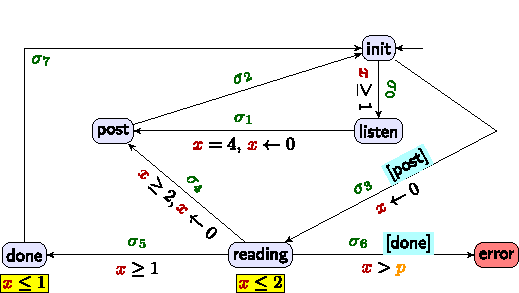
\includegraphics[width=0.95\linewidth,height=0.4\textheight,keepaspectratio]{graphic-01.pdf}\end{center}
 
Figure 1: Asynchronous data read example (variation from [13]).\par
 
% END S1.F1
 
% END S1.SSx1.SSS0.P0.SPx1
 
% BEGIN S1.SSx1.SSS0.P0.SPx2
 
\par\medskip\noindent\textbf{Problems.}\par
 
% BEGIN S1.SSx1.SSS0.P0.SPx2.p1
 
We focus here on the parametrised reachability-emptiness problem: decide the emptiness of the set of timing parameter valuations for which there exists a number of processes such that a given configuration is reachable.\par
 
% END S1.SSx1.SSS0.P0.SPx2.p1
 
% BEGIN S1.SSx1.SSS0.P0.SPx2.p2
 
We consider both local properties (reachability condition involving one process), and global properties (which can express the absence of deadlocks, or the fact that all processes must reach a given location).\par
 
% END S1.SSx1.SSS0.P0.SPx2.p2
 
% BEGIN S1.SSx1.SSS0.P0.SPx2.p3
 
We also distinguish the presence or the absence of invariants -- and we will see that this makes a critical difference in decidability.\par
 
% END S1.SSx1.SSS0.P0.SPx2.p3
 
% BEGIN S1.SSx1.SSS0.P0.SPx2.p4
 
In this paper, we prove several results regarding parametrised reachability-emptiness:\par
  
\par\noindent  $\blacksquare$ 
% BEGIN S1.I1.i1.p1
 
undecidability of local properties for PDTNs with 1 clock, 1 parameter, with invariants (Section 5.2).\par
 
% END S1.I1.i1.p1
 
 
\par\noindent  $\blacksquare$ 
% BEGIN S1.I1.i2.p1
 
undecidability of global properties for PDTNs with 1 clock, 1 parameter, with or without invariants (Section 5.3).\par
 
% END S1.I1.i2.p1
 
 
\par\noindent  $\blacksquare$ 
% BEGIN S1.I1.i3.p1
 
decidability for fully parametric PDTNs with 1 parameter (Section 6.1);\par
 
% END S1.I1.i3.p1
 
 
\par\noindent  $\blacksquare$ 
% BEGIN S1.I1.i4.p1
 
decidability for PDTNs when parameters are partitioned into lower-bound and upper-bound parameters (Section 6.2);\par
 
% END S1.I1.i4.p1
 
 
\par\noindent  $\blacksquare$ 
% BEGIN S1.I1.i5.p1
 
decidability of local properties for PDTNs with 1 clock, arbitrarily many parameters, without invariants (Section 6.3).\par
 
% END S1.I1.i5.p1
 
  
The most surprising result emphasizes the high expressive power of invariants (something which has no impact in single PTAs): local properties in PDTNs are decidable without invariants but become undecidable in their presence, for only 1 clock. In addition, both local and global properties are undecidable with invariants for a single clock and a single parameter -- a setting decidable in the context of PTAs taken in isolation: that is to say, while the communication primitive is weak, it is sufficiently expressive to encode models such a 2-counter machines.\par
 
% END S1.SSx1.SSS0.P0.SPx2.p4
 
% BEGIN S1.SSx1.SSS0.P0.SPx2.p5
 
Additionally, both as a proof ingredient and as an interesting result per se, we show in Section 5.1 that the reachability-emptiness problem is undecidable for 1 clock, 1 parameter, with and without invariants and any a priori fixed number ($\geq 3$) of processes -- even though the parametrised version of this problem, i.e., for any (non a priori fixed) number of processes, is decidable.\par
 
% END S1.SSx1.SSS0.P0.SPx2.p5
 
% END S1.SSx1.SSS0.P0.SPx2
 
% BEGIN S1.SSx1.SSS0.P0.SPx3
 
\par\medskip\noindent\textbf{Related work.}\par
 
% BEGIN S1.SSx1.SSS0.P0.SPx3.p1
 
The concept of identical processes in a timed setting was mainly addressed in networks of processes that either communicate via $k$-wise synchronization [5, 4, 3] or via location guards [35, 12, 13]. The former model is equivalent to a variant of timed Petri nets [33, 31, 25, 20], whereas the latter would be equivalent to a form of timed Petri nets restricted to immediate observation steps (as in [23, 34]), which however have not been studied separately to the best of our knowledge.\par
 
% END S1.SSx1.SSS0.P0.SPx3.p1
 
% BEGIN S1.SSx1.SSS0.P0.SPx3.p2
 
Very few works study decidability results when combining two types of parameters, i.e., discrete (number of processes) and continuous (timing parameters). In [21, 30], security protocols are studied with unknown timing constants, and an unbounded number of participants. However, the focus is not on decidability, and the general setting is undecidable. In [15], action parameters (that can be seen as Boolean variables) and continuous timing parameters are combined (only linearly though) in an extension of PTAs; the mere emptiness of the sets of action and timing parameters for which a location is reachable is undecidable. In contrast, we exhibit in this work some decidable cases.\par
 
% END S1.SSx1.SSS0.P0.SPx3.p2
 
% BEGIN S1.SSx1.SSS0.P0.SPx3.p3
 
The closest work to ours, and presumably the only one to consider timing parameters in the setting of parametrised verification, is in [11] where parametric timed broadcast protocols (PTBPs) are introduced. Our contributions differ in the communication setting: while we consider location guards, [11] considers broadcast in cliques (in which every message reaches every process) and in reconfigurable topologies (in which the set of receivers is chosen non-deterministically). Moreover, in this work we study the power of invariants, which are absent from [11]. Our decidability results are also significantly better than in [11]: In [11], parametrised reachability-emptiness (for local properties) is undecidable for PTBPs composed of general PTAs, even with a single clock and without invariants, both in the reconfigurable semantics and in the clique semantics. The only decidable subcase (for both semantics) for reachability-emptiness in [11] is severely restricted with 3 conditions that must hold simultaneously: a single clock per process, parameters partitioned into lower-bound and upper-bound parameters, and bounded (possibly rational-valued) parameters -- relaxing any of these conditions leads to undecidability. In contrast, we prove here decidability for general PDTNs with 1 clock and arbitrarily many parameters, or for parameters partitioned into lower-bound and upper-bound. Also note that our results do not reuse any proof ingredients from [11] due to the different communication.\par
 
% END S1.SSx1.SSS0.P0.SPx3.p3
 
% END S1.SSx1.SSS0.P0.SPx3
 
% BEGIN S1.SSx1.SSS0.P0.SPx4
 
\par\medskip\noindent\textbf{Outline.}\par
 
% BEGIN S1.SSx1.SSS0.P0.SPx4.p1
 
We recall the necessary material in Section 2. We formalize parametric disjunctive timed networks in Section 3, and our problem in Section 4. We prove undecidability results in Section 5 and decidability results in Section 6. We conclude in Section 7.\par
 
% END S1.SSx1.SSS0.P0.SPx4.p1
 
% END S1.SSx1.SSS0.P0.SPx4
 
% END S1.SSx1
 
% END S1


% BEGIN S2
 
\par\medskip\noindent\textbf{2 Parametric timed automata}\par
 
% BEGIN S2.p1
 
We denote by $\mathbb{N},\mathbb{N}_{>0},\mathbb{Z},\mathbb{R}_{\geq 0}$ the sets of non-negative integers, strictly positive integers, integers, and non-negative reals, respectively.\par
 
% END S2.p1
 
% BEGIN S2.p2
 
Clocks are real-valued variables that all evolve over time at the same rate. Throughout this paper, we assume a set $\mathbb{X}=\{x_{1},\dots,x_{H}\}$ of clocks. A clock valuation is a function $\mu:\mathbb{X}\to\mathbb{R}_{\geq 0}$, assigning a non-negative value to each clock. We write $\vec{0}$ for the clock valuation assigning $0$ to all clocks. Given $R\subseteq\mathbb{X}$, we define the reset of a valuation $\mu$, denoted by $[\mu]_{R}$, as follows: $[\mu]_{R}(x)=0$ if $x\in R$, and $[\mu]_{R}(x)=\mu(x)$ otherwise. Given a constant $d\in\mathbb{R}_{\geq 0}$, $\mu+d$ denotes the valuation s.t. $(\mu+d)(x)=\mu(x)+d$, for all $x\in\mathbb{X}$.\par
 
% END S2.p2
 
% BEGIN S2.p3
 
A (timing) parameter is an unknown integer-valued constant. Throughout this paper, we assume a set $\mathbb{P}=\{p_{1},\dots,p_{M}\}$ of parameters. A parameter valuation $v$ is a function $v:\mathbb{P}\to\mathbb{N}$.\par
 
% END S2.p3
 
% BEGIN S2.p4
 
A constraint $C$ is a conjunction of inequalities over $\mathbb{X}\cup\mathbb{P}$ of the form $x\bowtie\sum_{1\leq i\leq M}\alpha_{i}\times p_{i}+d$, with $x\in\mathbb{X}$, ${\bowtie}\in\{<,\leq,=,\geq,>\}$, $p_{i}\in\mathbb{P}$, and $\alpha_{i},d\in\mathbb{Z}$. We call $d$ a constant term. Given $C$, we write $\mu\models v(C)$ if the expression obtained by replacing each $x$ with $\mu(x)$ and each $p_{i}$ with $v(p_{i})$ in $C$ evaluates to true. Let $\Phi(\mathbb{X}\cup\mathbb{P})$ denote the set of constraints over $\mathbb{X}\cup\mathbb{P}$. Let $\mathit{True}$ denote the constraint made of no inequality, i.e., representing the whole set of clock and parameter valuations.\par
 
% END S2.p4
 
% BEGIN Thmtheorem1
 
\par\medskip\noindent\textbf{Definition 1 (PTA [8]).}\par
 
% BEGIN Thmtheorem1.p1
 
A PTA $\mathcal{A}$ is a tuple $\mathcal{A}=(\Sigma,L,\mathrm{\mathrm{\ell}_{0}},\mathbb{X},\mathbb{P},I,E)$, where:\par
  
\par\noindent  1) 
% BEGIN S2.I1.i1.p1
 
$\Sigma$ is a finite set of actions;\par
 
% END S2.I1.i1.p1
 
 
\par\noindent  2) 
% BEGIN S2.I1.i2.p1
 
$L$ is a finite set of locations;\par
 
% END S2.I1.i2.p1
 
 
\par\noindent  3) 
% BEGIN S2.I1.i3.p1
 
$\mathrm{\mathrm{\ell}_{0}}\in L$ is the initial location;\par
 
% END S2.I1.i3.p1
 
 
\par\noindent  4) 
% BEGIN S2.I1.i4.p1
 
$\mathbb{X}$ is a finite set of clocks;\par
 
% END S2.I1.i4.p1
 
 
\par\noindent  5) 
% BEGIN S2.I1.i5.p1
 
$\mathbb{P}$ is a finite set of parameters;\par
 
% END S2.I1.i5.p1
 
 
\par\noindent  6) 
% BEGIN S2.I1.i6.p1
 
$I:L\to\Phi(\mathbb{X}\cup\mathbb{P})$ is the invariant, assigning to every $\mathrm{\ell}\in L$ a constraint $I(\mathrm{\ell})$ over $\mathbb{X}\cup\mathbb{P}$;\par
 
% END S2.I1.i6.p1
 
 
\par\noindent  7) 
% BEGIN S2.I1.i7.p1
 
$E\subseteq L\times\Phi(\mathbb{X}\cup\mathbb{P})\times\Sigma\times 2^{\mathbb{X}}\times L$ is a finite set of edges $\tau=(\mathrm{\ell},g,a,R,\mathrm{\ell}^{\prime})$ where $\mathrm{\ell},\mathrm{\ell}^{\prime}\in L$ are the source and target locations, $g$ is a constraint (called guard), $a\in\Sigma$, and $R\subseteq\mathbb{X}$ is a set of clocks to be reset.\par
 
% END S2.I1.i7.p1
 
  
We say that a location $\mathrm{\ell}$ does not have an invariant if $I(\mathrm{\ell})=\mathit{True}$.\par
 
% END Thmtheorem1.p1
 
% END Thmtheorem1
 
% BEGIN Thmtheorem2
 
\par\medskip\noindent\textbf{Definition 2 (Valuation of a PTA).}\par
 
% BEGIN Thmtheorem2.p1
 
Given a PTA $\mathcal{A}$ and a parameter valuation $v$, we denote by $v(\mathcal{A})$ the non-parametric structure where all occurrences of a parameter $p_{i}$ have been replaced by $v(p_{i})$. $v(\mathcal{A})$ is a timed automaton.\par
 
% END Thmtheorem2.p1
 
% END Thmtheorem2
 
% BEGIN S2.p5
 
We recall the concrete semantics of a TA using a timed transition system (TTS).\par
 
% END S2.p5
 
% BEGIN Thmtheorem3
 
\par\medskip\noindent\textbf{Definition 3 (Semantics of a TA).}\par
 
% BEGIN Thmtheorem3.p1
 
Given a PTA $\mathcal{A}=(\Sigma,L,\mathrm{\mathrm{\ell}_{0}},\mathbb{X},\mathbb{P},I,E)$ and a parameter valuation $v$, the semantics of $v(\mathcal{A})$ is given by the TTS $\mathfrak{T}_{v(\mathcal{A})}=(\mathfrak{S},\mathfrak{s}_{0},\Sigma\cup\mathbb{R}_{\geq 0},{\rightarrow})$, with\par
  
\par\noindent  1. 
% BEGIN S2.I2.i1.p1
 
$\mathfrak{S}=\big\{(\mathrm{\ell},\mu)\in L\times\mathbb{R}_{\geq 0}^{H}\mid\mu\models v(I(\mathrm{\ell}))\big\}$, $\mathfrak{s}_{0}=(\mathrm{\mathrm{\ell}_{0}},\vec{0})$,\par
 
% END S2.I2.i1.p1
 
 
\par\noindent  2. 
% BEGIN S2.I2.i2.p1
 
${\rightarrow}$ consists of the discrete and (continuous) delay transition relations:\par
  
\par\noindent  (a) 
% BEGIN S2.I2.i2.I1.i1.p1
 
discrete transitions: $(\mathrm{\ell},\mu)\stackrel{{\scriptstyle\tau}}{{\mapsto}}(\mathrm{\ell}^{\prime},\mu^{\prime})$, if $(\mathrm{\ell},\mu),(\mathrm{\ell}^{\prime},\mu^{\prime})\in\mathfrak{S}$, and there exists $\tau=(\mathrm{\ell},g,a,R,\mathrm{\ell}^{\prime})\in E$, such that $\mu^{\prime}=[\mu]_{R}$, and $\mu\models v(g$).\par
 
% END S2.I2.i2.I1.i1.p1
 
 
\par\noindent  (b) 
% BEGIN S2.I2.i2.I1.i2.p1
 
delay transitions: $(\mathrm{\ell},\mu)\stackrel{{\scriptstyle d}}{{\mapsto}}(\mathrm{\ell},\mu+d)$, with $d\in\mathbb{R}_{\geq 0}$, if $\forall d^{\prime}\in[0,d],(\mathrm{\ell},\mu+d^{\prime})\in\mathfrak{S}$.\par
 
% END S2.I2.i2.I1.i2.p1
 
  
% END S2.I2.i2.p1
 
  
% END Thmtheorem3.p1
 
% END Thmtheorem3
 
% BEGIN S2.p6
 
Moreover we write $(\mathrm{\ell},\mu)\stackrel{{\scriptstyle(d,\tau)}}{{\longrightarrow}}(\mathrm{\ell}^{\prime},\mu^{\prime})$ for a combination of a delay and a discrete transition if $\exists\mu^{\prime\prime}:(\mathrm{\ell},\mu)\stackrel{{\scriptstyle d}}{{\mapsto}}(\mathrm{\ell},\mu^{\prime\prime})\stackrel{{\scriptstyle\tau}}{{\mapsto}}(\mathrm{\ell}^{\prime},\mu^{\prime})$.\par
 
% END S2.p6
 
% BEGIN S2.p7
 
Given a TA ${A}$ with concrete semantics $\mathfrak{T}_{{A}}$, we refer to the states of $\mathfrak{S}$ as the concrete states of ${A}$. A run of ${A}$ is an alternating sequence of concrete states of ${A}$ and pairs of delays and edges starting from the initial state $\mathfrak{s}_{0}$ of the form $(\mathrm{\mathrm{\ell}}_{0},\mu_{0}),(d_{0},\tau_{0}),(\mathrm{\mathrm{\ell}}_{1},\mu_{1}),\cdots$ with $i=0,1,\dots$, $\tau_{i}\in E$, $d_{i}\in\mathbb{R}_{\geq 0}$ and $(\mathrm{\mathrm{\ell}}_{i},\mu_{i})\stackrel{{\scriptstyle(d_{i},\tau_{i})}}{{\longrightarrow}}(\mathrm{\mathrm{\ell}}_{i+1},\mu_{i+1})$. Given a TA ${A}$, we say that a location $\mathrm{\ell}$ is reachable if there exists a state $(\mathrm{\ell},\mu)$ that appears on a run of ${A}$.\par
 
% END S2.p7
 
% BEGIN S2.SS0.SSS0.P0.SPx1
 
\par\medskip\noindent\textbf{Reachability-emptiness.}\par
 
% BEGIN S2.SS0.SSS0.P0.SPx1.p1
 
Given a PTA $\mathcal{A}$ and a location $\mathrm{\ell}$, the reachability-emptiness problem asks whether the set of parameter valuations $v$ such that $\mathrm{\ell}$ is reachable in $v(\mathcal{A})$ is empty.\par
 
% END S2.SS0.SSS0.P0.SPx1.p1
 
% BEGIN Thmtheorem4
 
\par\medskip\noindent\textbf{Definition 4 (L/U-PTA [27]).}\par
 
% BEGIN Thmtheorem4.p1
 
An L/U-PTA (lower-bound/upper-bound PTA) is a PTA where $\mathbb{P}$ is partitioned into $\mathbb{P}=\mathbb{P}_{L}\uplus\mathbb{P}_{U}$, where $\mathbb{P}_{L}$ (resp. $\mathbb{P}_{U}$) denotes lower-bound (resp. upper-bound) parameters, so that each lower-bound (resp. upper-bound) parameter $p_{i}$ must be such that, for every constraint $x\bowtie\sum_{1\leq i\leq M}\alpha_{i}\times p_{i}+d$, we have:\par
  
\par\noindent  1) 
% BEGIN S2.I3.i1.p1
 
${\bowtie}\in\left\{\leq,<\right\}$ implies $\alpha_{i}\leq 0$ (resp. $\alpha_{i}\geq 0$), and\par
 
% END S2.I3.i1.p1
 
 
\par\noindent  2) 
% BEGIN S2.I3.i2.p1
 
${\bowtie}\in\left\{\geq,>\right\}$ implies $\alpha_{i}\geq 0$ (resp. $\alpha_{i}\leq 0$).\par
 
% END S2.I3.i2.p1
 
  
% END Thmtheorem4.p1
 
% END Thmtheorem4
 
% BEGIN S2.SS0.SSS0.P0.SPx1.p2
 
A PTA is fully parametric whenever it has no constant term (apart from 0):\par
 
% END S2.SS0.SSS0.P0.SPx1.p2
 
% BEGIN Thmtheorem5
 
\par\medskip\noindent\textbf{Definition 5 (Fully parametric PTA [27, Definition 4.6]).}\par
 
% BEGIN Thmtheorem5.p1
 
A PTA $\mathcal{A}$ is fully parametric if every constraint in $\mathcal{A}$ is of the form $x\bowtie\sum_{1\leq i\leq M}\alpha_{i}\times p_{i}$, with $p_{i}\in\mathbb{P}$ and $\alpha_{i}\in\mathbb{Z}$.\par
 
% END Thmtheorem5.p1
 
% END Thmtheorem5
 
% BEGIN S2.SS0.SSS0.P0.SPx1.p3
 
Our subsequent undecidability proofs work by reduction from the halting problem for 2-counter machines. We borrow the following material from [17]. A deterministic 2-counter machine (“2CM”) [32] has two non-negative counters $\mathcal{C}_{1}$ and $\mathcal{C}_{2}$, a finite number of states and a finite number of transitions, which can be of the form (for $l\in\{1,2\}$):\par
  
\par\noindent  i) 
% BEGIN S2.I4.i1.p1
 
“when in state $\mathtt{q}_{i}$, increment $\mathcal{C}_{l}$ and go to $\mathtt{q}_{j}$”; or\par
 
% END S2.I4.i1.p1
 
 
\par\noindent  ii) 
% BEGIN S2.I4.i2.p1
 
“when in state $\mathtt{q}_{i}$, if $\mathcal{C}_{l}=0$ then go to $\mathtt{q}_{k}$, otherwise decrement $\mathcal{C}_{l}$ and go to $\mathtt{q}_{j}$”.\par
 
% END S2.I4.i2.p1
 
  
% END S2.SS0.SSS0.P0.SPx1.p3
 
% BEGIN S2.SS0.SSS0.P0.SPx1.p4
 
The 2CM starts in state $\mathtt{q}_{0}$ with the counters set to 0. The machine follows a deterministic transition function, meaning for each combination of state and counter conditions, there is exactly one action to take. The halting problem consists in deciding whether some distinguished state called $\mathtt{q}_{\textrm{halt}}$ can be reached or not. This problem is known to be undecidable [32].\par
 
% END S2.SS0.SSS0.P0.SPx1.p4
 
% END S2.SS0.SSS0.P0.SPx1
 
% END S2


% BEGIN S3
 
\par\medskip\noindent\textbf{3 Parametric disjunctive timed networks}\par
 
% BEGIN S3.p1
 
We extend guarded TAs defined in [12] with timing parameters as in PTAs. We follow the terminology and use abbreviations from [35, 12].\par
 
% END S3.p1
 
% BEGIN Thmtheorem6
 
\par\medskip\noindent\textbf{Definition 6 (Guarded Parametric Timed Automaton (gPTA)).}\par
 
% BEGIN Thmtheorem6.p1
 
A gPTA $\mathcal{A}$ is a tuple $\mathcal{A}=(\Sigma,L,\mathrm{\mathrm{\ell}_{0}},\mathbb{X},\mathbb{P},I,E)$, where:\par
  
\par\noindent  1) 
% BEGIN S3.I1.i1.p1
 
$\Sigma$ is a finite set of actions;\par
 
% END S3.I1.i1.p1
 
 
\par\noindent  2) 
% BEGIN S3.I1.i2.p1
 
$L$ is a finite set of locations;\par
 
% END S3.I1.i2.p1
 
 
\par\noindent  3) 
% BEGIN S3.I1.i3.p1
 
$\mathrm{\mathrm{\ell}_{0}}\in L$ is the initial location;\par
 
% END S3.I1.i3.p1
 
 
\par\noindent  4) 
% BEGIN S3.I1.i4.p1
 
$\mathbb{X}$ is a finite set of clocks;\par
 
% END S3.I1.i4.p1
 
 
\par\noindent  5) 
% BEGIN S3.I1.i5.p1
 
$\mathbb{P}$ is a finite set of parameters;\par
 
% END S3.I1.i5.p1
 
 
\par\noindent  6) 
% BEGIN S3.I1.i6.p1
 
$I:L\to\Phi(\mathbb{X}\cup\mathbb{P})$ is the invariant, assigning to every $\mathrm{\ell}\in L$ a constraint $I(\mathrm{\ell})$ (called invariant);\par
 
% END S3.I1.i6.p1
 
 
\par\noindent  7) 
% BEGIN S3.I1.i7.p1
 
$E\subseteq L\times\Phi(\mathbb{X}\cup\mathbb{P})\times\left(L\cup\{\top\}\right)\times\Sigma\times 2^{\mathbb{X}}\times L$ is a finite set of edges $\tau=(\mathrm{\ell},g,\gamma,a,R,\mathrm{\ell}^{\prime})$ where $\mathrm{\ell},\mathrm{\ell}^{\prime}\in L$ are the source and target locations, $g$ is a constraint (called guard), $\gamma$ is the location guard, $a\in\Sigma$, and $R\subseteq\mathbb{X}$ is a set of clocks to be reset.\par
 
% END S3.I1.i7.p1
 
  
% END Thmtheorem6.p1
 
% END Thmtheorem6
 
% BEGIN S3.p2
 
Intuitively, an edge $\tau=(\mathrm{\ell},g,\gamma,a,R,\mathrm{\ell}^{\prime})\in E$ takes the automaton from location $\mathrm{\ell}$ to $\mathrm{\ell}^{\prime}$; $\tau$ can only be taken if guard $g$ and location guard $\gamma$ are both satisfied, and it resets all clocks in $R$. Note that satisfaction of location guards is only meaningful in a network of gPTAs (defined below). Intuitively, a location guard $\gamma$ is satisfied if it is $\top$ or if another automaton in the network currently occupies location $\gamma$.\par
 
% END S3.p2
 
% BEGIN Thmtheorem7
 
\par\medskip\noindent\textbf{Example 7.}\par
 
% BEGIN Thmtheorem7.p1
 
In Figure 1, the transition to $\mathsf{error}$ is guarded both by a guard $x>p$ and by a location guard $[\mathsf{done}]$. In contrast, the location guard to $\mathsf{done}$ is $\top$ (and omitted in the figure), i.e., it can be taken without assumption on the location of other processes.\par
 
% END Thmtheorem7.p1
 
% END Thmtheorem7
 
% BEGIN S3.p3
 
A gPTA is an L/U-gPTA if parameters are partitioned into lower-bound and upper-bound parameters (as in Definition 4). A gPTA is fully parametric whenever it has no constant term (apart from 0) in its guards and invariants, similarly to Definition 5.\par
 
% END S3.p3
 
% BEGIN S3.SS0.SSS0.P0.SPx1
 
\par\medskip\noindent\textbf{Recalling the semantics of NTAs.}\par
 
% BEGIN S3.SS0.SSS0.P0.SPx1.p1
 
A gPTA with $\mathbb{P}=\emptyset$ is called a guarded timed automaton (gTA) [12]. Given a gPTA $\mathcal{A}$ and a parameter valuation $v$, we denote by $v(\mathcal{A})$ the non-parametric structure where all occurrences of a parameter $p_{i}$ have been replaced by $v(p_{i})$; $v(\mathcal{A})$ is a gTA.\par
 
% END S3.SS0.SSS0.P0.SPx1.p1
 
% BEGIN S3.SS0.SSS0.P0.SPx1.p2
 
Let ${A}$ be a gTA. We denote by ${{A}}^{n}$ the parallel composition ${A}\parallel\cdots\parallel{A}$ of $n$ copies of ${A}$, also called a network of timed automata (NTA) of size $n$. Each copy of ${A}$ in the NTA ${{A}}^{n}$ is called a process. A configuration $\mathfrak{c}$ of an NTA ${{A}}^{n}$ is a tuple $\mathfrak{c}=\big((\mathrm{\ell}_{1},\mu_{1}),\ldots,(\mathrm{\ell}_{n},\mu_{n})\big)$, where every $(\mathrm{\ell}_{i},\mu_{i})$ is a concrete state of ${A}$. The semantics of ${{A}}^{n}$ can be defined as a TTS $(\mathfrak{C},\hat{\mathfrak{c}},T)$, where $\mathfrak{C}$ denotes the set of all configurations of ${{A}}^{n}$, $\hat{\mathfrak{c}}$ is the unique initial configuration $(\mathrm{\mathrm{\ell}_{0}},\mathbf{0})^{n}$, and the transition relation $T$ is the union of the following delay and discrete transitions:\par
  delay transition  
% BEGIN S3.I2.ix1.p1
 
${\big((\mathrm{\ell}_{1},\mu_{1}),\ldots,(\mathrm{\ell}_{n},\mu_{n})\big)}\xrightarrow{d}{\big((\mathrm{\ell}_{1},\mu_{1}+d),\ldots,(\mathrm{\ell}_{n},\mu_{n}+d)\big)}$, with $d\in\mathbb{R}_{\geq 0}$, if $\forall i\in\{1,\dots,n\},\forall d^{\prime}\in[0,d]:\mu_{i}+d^{\prime}\models
I(\mathrm{\ell}_{i})$, i.e., we can delay $d\in\mathbb{R}_{\geq 0}$ units of time if all clock invariants are satisfied until the end of the delay.\par
 
% END S3.I2.ix1.p1
  discrete transition  
% BEGIN S3.I2.ix2.p1
 
${\big((\mathrm{\ell}_{1},\mu_{1}),\ldots,(\mathrm{\ell}_{n},\mu_{n})\big)}\xrightarrow{(i,a)}{\big((\mathrm{\ell}_{1}^{\prime},\mu_{1}^{\prime}),\ldots,(\mathrm{\ell}_{n}^{\prime},\mu_{n}^{\prime})\big)}$ for some $i\in\{1,\dots,n\}$ if\par
  
\par\noindent  1) 
% BEGIN S3.I2.ix2.I0.i1.p1
 
${(\mathrm{\ell}_{i},\mu_{i})}\xrightarrow{\tau}{(\mathrm{\ell}_{i}^{\prime},\mu_{i}^{\prime})}$ is a discrete transition\footnote{11Strictly speaking, ${(\mathrm{\ell}_{i},\mu_{i})}\xrightarrow{\tau}{(\mathrm{\ell}_{i}^{\prime},\mu_{i}^{\prime})}$ is a transition of the TA obtained from ${A}$ by replacing location guards with $\top$. } of ${A}$ with $\tau=(\mathrm{\ell}_{i},g,\gamma,a,R,\mathrm{\ell}_{i}^{\prime})$ for some $g$, $\gamma$ and $R$,\par
 
% END S3.I2.ix2.I0.i1.p1
 
 
\par\noindent  2) 
% BEGIN S3.I2.ix2.I0.i2.p1
 
$\gamma=\top$ or $\mathrm{\ell}_{j}=\gamma$ for some $j\in\{1,\dots,n\}\setminus\{i\}$, and\par
 
% END S3.I2.ix2.I0.i2.p1
 
 
\par\noindent  3) 
% BEGIN S3.I2.ix2.I0.i3.p1
 
$\mathrm{\ell}_{j}^{\prime}=\mathrm{\ell}_{j}$ and $\mu_{j}^{\prime}=\mu_{j}$ for all $j\in\{1,\dots,n\}\setminus\{i\}$.\par
 
% END S3.I2.ix2.I0.i3.p1
 
  
% END S3.I2.ix2.p1
   
% END S3.SS0.SSS0.P0.SPx1.p2
 
% BEGIN S3.SS0.SSS0.P0.SPx1.p3
 
That is, location guards $\gamma$ are interpreted as disjunctive guards: unless $\gamma=\top$, at least one of the other processes needs to occupy location $\gamma$ in order for process $i$ to pass this guard.\par
 
% END S3.SS0.SSS0.P0.SPx1.p3
 
% BEGIN S3.SS0.SSS0.P0.SPx1.p4
 
We write ${\mathfrak{c}}\xrightarrow{d,(i,a)}{\mathfrak{c}^{\prime\prime}}$ for a delay transition ${\mathfrak{c}}\xrightarrow{d}{\mathfrak{c}^{\prime}}$ followed by a discrete transition ${\mathfrak{c}^{\prime}}\xrightarrow{(i,a)}{\mathfrak{c}^{\prime\prime}}$. Then, a timed path of ${{A}}^{n}$ is a finite sequence $\pi=\mathfrak{c}_{0}\xrightarrow{d_{0},(i_{0},a_{0})}\cdots\xrightarrow{d_{l-1},(i_{l-1},a_{l-1})}\mathfrak{c}_{l}$. A timed path $\pi$ of ${{A}}^{n}$ is a computation if $\mathfrak{c}_{0}=\hat{\mathfrak{c}}$. We say that $\mathfrak{c}_{l}$ is reachable in ${{A}}^{n}$.\par
 
% END S3.SS0.SSS0.P0.SPx1.p4
 
% BEGIN S3.SS0.SSS0.P0.SPx1.p5
 
We write $\mathrm{\ell}\in\mathfrak{c}$ if $\mathfrak{c}=\big((\mathrm{\ell}_{1},\mu_{1}),\ldots,(\mathrm{\ell}_{n},\mu_{n})\big)$ and $\mathrm{\ell}=\mathrm{\ell}_{i}$ for some $i\in\{1,\dots,n\}$. We say that a location $\mathrm{\ell}$ is reachable in ${{A}}^{n}$ if there exists a reachable configuration $\mathfrak{c}$ s.t. $\mathrm{\ell}\in\mathfrak{c}$.\par
 
% END S3.SS0.SSS0.P0.SPx1.p5
 
% BEGIN S3.SS0.SSS0.P0.SPx1.p6
 
Given a gPTA $\mathcal{A}$, we denote by ${\mathcal{A}}^{n}$ the parallel composition $\mathcal{A}\parallel\cdots\parallel\mathcal{A}$ of $n$ copies of $\mathcal{A}$, also called a network of parametric timed automata (NPTA). Given an NPTA ${\mathcal{A}}^{n}$ and a parameter valuation $v$, we denote by $v({\mathcal{A}}^{n})$ the non-parametric structure where all occurrences of a parameter $p_{i}$ have been replaced by $v(p_{i})$; note that $v({\mathcal{A}}^{n})$ is an NTA.\par
 
% END S3.SS0.SSS0.P0.SPx1.p6
 
% BEGIN Thmtheorem8
 
\par\medskip\noindent\textbf{Definition 8.}\par
 
% BEGIN Thmtheorem8.p1
 
A given gPTA $\mathcal{A}$ induces a parametric disjunctive timed network (PDTN) ${\mathcal{A}}^{\infty}$, defined as the following family of NPTAs: ${\mathcal{A}}^{\infty}=\{{\mathcal{A}}^{n}\mid n\in\mathbb{N}_{>0}\}$.\par
 
% END Thmtheorem8.p1
 
% END Thmtheorem8
 
% BEGIN S3.SS0.SSS0.P0.SPx1.p7
 
Given a parametric disjunctive timed network ${\mathcal{A}}^{\infty}$ and a parameter valuation $v$, ${(v(\mathcal{A}))}^{\infty}$ is a disjunctive timed network (DTN) [35].\par
 
% END S3.SS0.SSS0.P0.SPx1.p7
 
% BEGIN S3.SS0.SSS0.P0.SPx1.p8
 
Given a location $\mathrm{\ell}$ of a gPTA $\mathcal{A}$, given a parameter valuation $v$, we say that $\mathrm{\ell}$ is reachable in the DTN ${(v(\mathcal{A}))}^{\infty}$ if there exists $n\in\mathbb{N}_{>0}$ such that $\mathrm{\ell}$ is reachable in ${(v(\mathcal{A}))}^{n}$.\par
 
% END S3.SS0.SSS0.P0.SPx1.p8
 
% END S3.SS0.SSS0.P0.SPx1
 
% BEGIN S3.SS0.SSS0.P0.SPx2
 
\par\medskip\noindent\textbf{Subclasses of PDTNs.}\par
 
% BEGIN S3.SS0.SSS0.P0.SPx2.p1
 
A PDTN ${\mathcal{A}}^{\infty}$ induced by a gPTA $\mathcal{A}$ is an L/U-PDTN if $\mathcal{A}$ is an L/U-gPTA. Similarly, ${\mathcal{A}}^{\infty}$ is a fully parametric PDTN if $\mathcal{A}$ is a fully parametric gPTA.\par
 
% END S3.SS0.SSS0.P0.SPx2.p1
 
% END S3.SS0.SSS0.P0.SPx2
 
% END S3


% BEGIN S4
 
\par\medskip\noindent\textbf{4 Problems for parametric disjunctive timed networks}\par
 
% BEGIN S4.SS0.SSS0.P0.SPx1
 
\par\medskip\noindent\textbf{Reachability.}\par
 
% BEGIN S4.SS0.SSS0.P0.SPx1.p1
 
In [12], the parametrised reachability problem (PR) consists in deciding whether, given a gTA ${A}$ and a location $\mathrm{\ell}$, there exists $n\in\mathbb{N}$ such that $\mathrm{\ell}$ is reachable in ${{A}}^{n}$. Here, we consider a parametric version. The emptiness extension consists in asking whether the set of timing parameter valuations for which PR holds is empty.\par
 
% END S4.SS0.SSS0.P0.SPx1.p1
 
% BEGIN S4.SS0.SSS0.P0.SPx1.p2
 
Parameterized reachability-emptiness problem (PR-e): Input: a gPTA $\mathcal{A}$ and a location $\mathrm{\ell}$ Problem: Decide the emptiness of the set of timing parameter valuations $v$ for which $\mathrm{\ell}$ is reachable in ${(v(\mathcal{A}))}^{\infty}$.\par
 
% END S4.SS0.SSS0.P0.SPx1.p2
 
% BEGIN Thmtheorem9
 
\par\medskip\noindent\textbf{Example 9.}\par
 
% BEGIN Thmtheorem9.p1
 
In Figure 1, PR-e with $\mathsf{error}$ as target location does not hold: for $v(p)=1$, location $\mathsf{error}$ can be reached for $\geq 3$ processes.\par
 
% END Thmtheorem9.p1
 
% END Thmtheorem9
 
% BEGIN S4.SS0.SSS0.P0.SPx1.p3
 
Without invariants, $|L|$ is a cutoff (i.e., a number of processes above which the reachability is homogeneous -- better cutoffs are known for local properties). Intuitively, this is because, without invariants, a single process that reaches such a location can stay there and enable the guard forever. However, with invariants, such a simple cutoff does not work (even in the absence of timing parameters), since invariants might force a process to leave a location and lots of different processes might be needed to occupy a location at different points in time.\par
 
% END S4.SS0.SSS0.P0.SPx1.p3
 
% END S4.SS0.SSS0.P0.SPx1
 
% BEGIN S4.SS0.SSS0.P0.SPx2
 
\par\medskip\noindent\textbf{Global reachability.}\par
 
% BEGIN S4.SS0.SSS0.P0.SPx2.p1
 
Global properties refer to the numbers of processes in given locations; we express these using constraints. Formally, a global reachability property is defined by a constraint $\varphi$ in the following grammar: $\varphi::=\#\mathrm{\ell}\geq 1\mid\#\mathrm{\ell}=0\mid\varphi\land\varphi\mid\varphi\lor\varphi$, where $\mathrm{\ell}\in L$ and $\#\mathrm{\ell}$ refers to the number of processes in $\mathrm{\ell}$. Note that the “$\#\mathrm{\ell}=0$” term is responsible for the “global” nature of such properties, i.e., it must hold for all processes that they are not in $\mathrm{\ell}$. The satisfaction of a constraint $\varphi$ by $\mathfrak{c}=\big((\mathrm{\ell}_{1},\mu_{1}),\ldots,(\mathrm{\ell}_{n},\mu_{n})\big)$ is defined naturally: $\mathfrak{c}\models\#\mathrm{\ell}\geq 1$ if $\mathrm{\ell}\in\mathfrak{c}$; $\mathfrak{c}\models\#\mathrm{\ell}=0$ if $\mathrm{\ell}\notin\mathfrak{c}$; and as usual for Boolean combinations. The parametrised global reachability problem (PGR) consists in deciding whether, given a gTA ${A}$ and a global reachability property $\varphi$, there exists $n\in\mathbb{N}$ such that a configuration $\mathfrak{c}$ with $\mathfrak{c}\models\varphi$ is reachable in ${{A}}^{n}$. Again, we extend this problem to the emptiness of the set of timing parameters:\par
 
% END S4.SS0.SSS0.P0.SPx2.p1
 
% BEGIN S4.SS0.SSS0.P0.SPx2.p2
 
Parameterized global reachability-emptiness problem (PGR-e): Input: a gPTA $\mathcal{A}$ and a global reachability property $\varphi$ Problem: Decide the emptiness of the set of timing parameter valuations $v$ for which a configuration $\mathfrak{c}$ with $\mathfrak{c}\models\varphi$ is reachable in ${(v(\mathcal{A}))}^{\infty}$.\par
 
% END S4.SS0.SSS0.P0.SPx2.p2
 
% BEGIN S4.SS0.SSS0.P0.SPx2.p3
 
As special cases, the parametrised global reachability problem includes control-state reachability (where $\varphi$ is $\#\mathrm{\ell}\geq 1$ for a single location $\mathrm{\ell}$; also expressible as a PR-e problem) and detection of timelocks that are due to location guards (where $\varphi$ is a disjunction over conjunctions of the form $\#\mathrm{\ell}\geq 1\land\#\mathrm{\ell}_{1}=0\land\cdots\land\#\mathrm{\ell}_{m}=0$, where $\mathrm{\ell}$ can only be left through edges guarded by one of the $\mathrm{\ell}_{1},\ldots,\mathrm{\ell}_{m}$). We will be particularly interested in the global property asking whether all processes reach a given final configuration (where $\varphi$ is of the form $\#\mathrm{\ell}_{1}=0\land\cdots\land\#\mathrm{\ell}_{m}=0$ with $m=|L|-1$), sometimes called the target problem [22].\par
 
% END S4.SS0.SSS0.P0.SPx2.p3
 
% BEGIN Thmtheorem10
 
\par\medskip\noindent\textbf{Example 10.}\par
 
% BEGIN Thmtheorem10.p1
 
In Figure 1, consider the global property $\varphi$ stating that all processes must be in $\mathsf{error}$. This property can be written as $\#\mathsf{init}=0\land\#\mathsf{listen}=0\land\#\mathsf{post}=0\land\#\mathsf{reading}=0\land\#\mathsf{done}=0$; then, PGR-e holds: no parameter valuation can allow all processes to be simultaneously in $\mathsf{error}$, whatever the number of processes (this comes from the fact that the transition to $\mathsf{error}$ is guarded by $\mathsf{done}$, so at least one process must be elsewhere).\par
 
% END Thmtheorem10.p1
 
% END Thmtheorem10
 
% END S4.SS0.SSS0.P0.SPx2
 
% END S4


% BEGIN S5
 
\par\medskip\noindent\textbf{5 Undecidability results}\par
 
% BEGIN S5.SS1
 
\par\medskip\noindent\textbf{5.1 Fixed number of processes}\par
 
% BEGIN S5.SS1.p1
 
We first consider a fixed number of processes; the problem addressed here is therefore not (yet) parametrised reachability-emptiness, but only reachability-emptiness. These results will be used as important proof ingredients for the results in Sections 5.2 and 5.3. (Then, the three results in Section 6 use 3 different proof techniques, completely different from this one.)\par
 
% END S5.SS1.p1
 
% BEGIN S5.SS1.SSS1
 
\par\medskip\noindent\textbf{5.1.1 Undecidability for 3 processes}\par
 
% BEGIN S5.SS1.SSS1.p1
 
In the following, we show that the emptiness of the parameter valuations set for which a location is reachable in an NPTA made of exactly 3 processes (“reachability-emptiness”) is undecidable. We first prove the result with invariants (Proposition 13), and then show it also holds without (Proposition 14). The idea is that invariants are not needed for 3 processes, but will be necessary when proving undecidability for an unbounded number of processes (Theorem 16).\par
 
% END S5.SS1.SSS1.p1
 
% BEGIN S5.SS1.SSS1.p2
 
Before that, we first reprove a well-known result stating that reachability-emptiness is undecidable for PTAs with 3 clocks and a single parameter. This result was already proved (with 3 or more clocks) in, e.g., [8, 18, 16] with various proof flavors. The construction we introduce in the proof of Lemma 11 will be then reused and modified in the proof of Proposition 13, which is why we give it first with full details.\par
 
% END S5.SS1.SSS1.p2
 
% BEGIN S5.F2
   
% BEGIN S5.F2.sf1

\begin{center}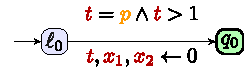
\includegraphics[width=0.95\linewidth,height=0.4\textheight,keepaspectratio]{graphic-02.pdf}\end{center}
 
(a) Initial gadget: single PTA version.\par
 
% END S5.F2.sf1
   
% BEGIN S5.F2.sf2

\begin{center}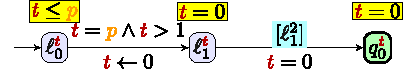
\includegraphics[width=0.95\linewidth,height=0.4\textheight,keepaspectratio]{graphic-03.pdf}\end{center}
 
(b) Initial gadget: gadget simulating $t$.\par
 
% END S5.F2.sf2
    
% BEGIN S5.F2.sf3

\begin{center}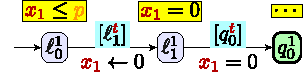
\includegraphics[width=0.95\linewidth,height=0.4\textheight,keepaspectratio]{graphic-04.pdf}\end{center}
 
(c) Initial gadget: gadget simulating $x_{1}$.\par
 
% END S5.F2.sf3
   
% BEGIN S5.F2.sf4

\begin{center}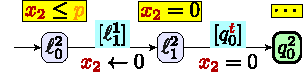
\includegraphics[width=0.95\linewidth,height=0.4\textheight,keepaspectratio]{graphic-05.pdf}\end{center}
 
(d) Initial gadget: gadget simulating $x_{2}$.\par
 
% END S5.F2.sf4
    
% BEGIN S5.F2.sf5

\begin{center}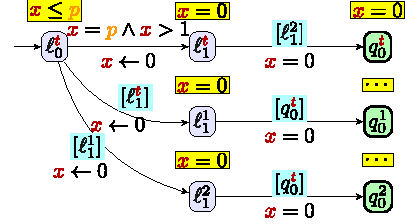
\includegraphics[width=0.95\linewidth,height=0.4\textheight,keepaspectratio]{graphic-06.pdf}\end{center}
 
(e) Initial gadget: global gadget as a single gPTA.\par
 
% END S5.F2.sf5
   
% BEGIN S5.F2.sf6

\begin{center}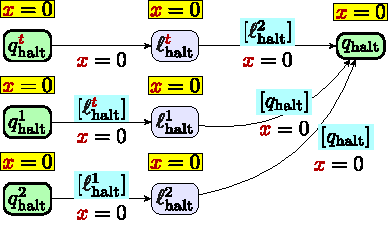
\includegraphics[width=0.95\linewidth,height=0.4\textheight,keepaspectratio]{graphic-07.pdf}\end{center}
 
(f) Final gadget as a single gPTA.\par
 
% END S5.F2.sf6
   
Figure 2: Initial and final gadgets.\par
 
% END S5.F2
 
% BEGIN Thmtheorem11
 
\par\medskip\noindent\textbf{Lemma 11.}\par
 
% BEGIN Thmtheorem11.p1
 
Reachability-emptiness is undecidable for PTAs with 3 clocks and 1 parameter.\par
 
% END Thmtheorem11.p1
 
% END Thmtheorem11
 
% BEGIN S5.SS1.SSS1.P0.SPx1
 
\par\medskip\noindent\textbf{Proof.}\par
 
% BEGIN S5.SS1.SSS1.P0.SPx1.p1
 
We reduce from the halting problem of 2-counter machines, which is undecidable [32]. Given a 2CM $\mathcal{M}$, we encode it as a PTA $\mathcal{A}$. Let us describe this encoding in detail, as we will modify it in the subsequent proofs.\par
 
% END S5.SS1.SSS1.P0.SPx1.p1
 
% BEGIN S5.SS1.SSS1.P0.SPx1.p2
 
Each state $\mathtt{q}_{i}$ of the machine is encoded as a location of the PTA, which we call $q_{i}$. The counters are encoded using clocks $t$, $x_{1}$ and $x_{2}$ and one integer-valued parameter $p$, with the following relations with the values $c_{1}$ and $c_{2}$ of counters $\mathcal{C}_{1}$ and $\mathcal{C}_{2}$: when $t=0$, we have $x_{1}=c_{1}$ and $x_{2}=c_{2}$. This clock encoding is classical for integer-valued parameters, e.g., [18, 16]. The parameter typically encodes the maximal value of the counters along a run.\par
 
% END S5.SS1.SSS1.P0.SPx1.p2
 
% BEGIN S5.SS1.SSS1.P0.SPx1.p3
 
We initialize the clocks with the gadget in Figure 2(a) (that also blocks the case where $p\leq 1$). Note that, throughout the paper, we highlight in thick green style the locations of the PTA corresponding to a state of the 2CM (in contrast with other locations added in the encoding to maintain the matching between the clock values and the counter values). Since all clocks are initially 0, in Figure 2(a) clearly, when in $q_{0}$ with $t=0$, we have $x_{1}=x_{2}=0$, which indeed corresponds to counter values $0$.\par
 
% END S5.SS1.SSS1.P0.SPx1.p3
 
% BEGIN S5.SS1.SSS1.P0.SPx1.p4
 
We now present the gadget encoding the increment instruction of $\mathcal{C}_{1}$ in Figure 3(a). The edge from $q_{i}$ to $\mathrm{\mathrm{\ell}}_{i1}$ only serves to clearly indicate the entry in the increment gadget and is done in $0$ time unit. Since every edge is guarded by one equality, there are really only two timed paths that go through the gadget: one going through $\mathrm{\mathrm{\ell}}_{i2}$ and one through $\mathrm{\mathrm{\ell}}_{i2}^{\prime}$, depending on the respective order between $c_{1}$ and $c_{2}$. Observe that on both timed paths the gadget lasts exactly $p$ time units (due to the guards and resets of $t$). In addition, $x_{2}$ is reset exactly when it equals $p$, hence its value when entering the gadget is identical to its value when reaching $q_{j}$. Therefore $c_{2}$ is unchanged. Now, $x_{1}$ is reset when it equals $p-1$, hence its value after the gadget of duration $p$ is incremented by 1 compared to its value when entering the gadget. Therefore $c_{1}$ is incremented by 1 when reaching $q_{j}$, as expected.\par
 
% END S5.SS1.SSS1.P0.SPx1.p4
 
% BEGIN S5.F3
   
% BEGIN S5.F3.sf1

\begin{center}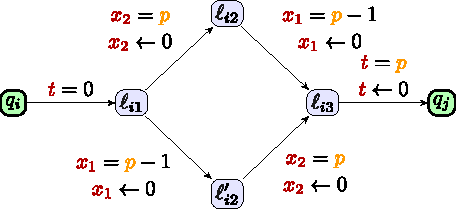
\includegraphics[width=0.95\linewidth,height=0.4\textheight,keepaspectratio]{graphic-08.pdf}\end{center}
 
(a) Increment $\mathcal{C}_{1}$: single PTA version.\par
 
% END S5.F3.sf1
   
% BEGIN S5.F3.sf2

\begin{center}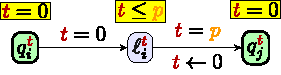
\includegraphics[width=0.95\linewidth,height=0.4\textheight,keepaspectratio]{graphic-09.pdf}\end{center}
 
(b) Increment $\mathcal{C}_{1}$: gadget simulating $t$.\par
 
% END S5.F3.sf2
    
% BEGIN S5.F3.sf3

\begin{center}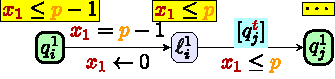
\includegraphics[width=0.95\linewidth,height=0.4\textheight,keepaspectratio]{graphic-10.pdf}\end{center}
 
(c) Increment $\mathcal{C}_{1}$: gadget simulating $x_{1}$.\par
 
% END S5.F3.sf3
   
% BEGIN S5.F3.sf4

\begin{center}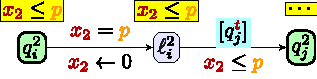
\includegraphics[width=0.95\linewidth,height=0.4\textheight,keepaspectratio]{graphic-11.pdf}\end{center}
 
(d) Increment $\mathcal{C}_{1}$: gadget simulating $x_{2}$.\par
 
% END S5.F3.sf4
   
Figure 3: Increment gadget.\par
 
% END S5.F3
 
% BEGIN S5.F4
   
% BEGIN S5.F4.sf1

\begin{center}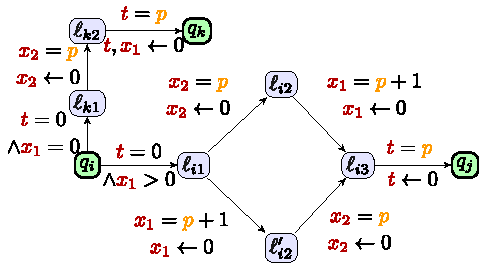
\includegraphics[width=0.95\linewidth,height=0.4\textheight,keepaspectratio]{graphic-12.pdf}\end{center}
 
(a) 0-test and decrement ($\mathcal{C}_{1}$): single PTA version.\par
 
% END S5.F4.sf1
   
% BEGIN S5.F4.sf2

\begin{center}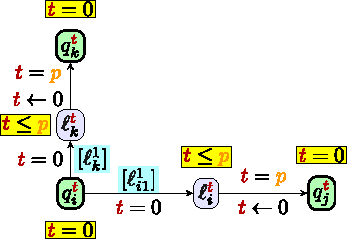
\includegraphics[width=0.95\linewidth,height=0.4\textheight,keepaspectratio]{graphic-13.pdf}\end{center}
 
(b) 0-test and decrement ($\mathcal{C}_{1}$): gadget simulating $t$.\par
 
% END S5.F4.sf2
    
% BEGIN S5.F4.sf3

\begin{center}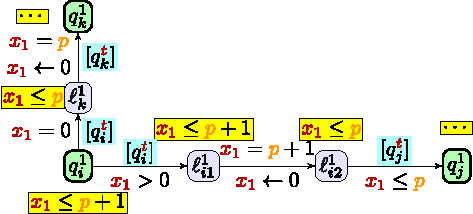
\includegraphics[width=0.95\linewidth,height=0.4\textheight,keepaspectratio]{graphic-14.pdf}\end{center}
 
(c) 0-test and decrement ($\mathcal{C}_{1}$): gadget simulating $x_{1}$.\par
 
% END S5.F4.sf3
   
% BEGIN S5.F4.sf4

\begin{center}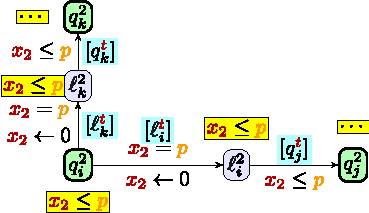
\includegraphics[width=0.95\linewidth,height=0.4\textheight,keepaspectratio]{graphic-15.pdf}\end{center}
 
(d) 0-test and decrement ($\mathcal{C}_{1}$): gadget simulating $x_{2}$.\par
 
% END S5.F4.sf4
   
Figure 4: 0-test and decrement gadget.\par
 
% END S5.F4
 
% BEGIN S5.SS1.SSS1.P0.SPx1.p5
 
Let us now consider the 0-test and decrement gadget. Decrement is done similarly to increment, by replacing guards $x_{1}=p-1$ with $x_{1}=p+1$, as shown in Figure 4(a). In addition, the 0-test is obtained by simply testing that $x_{1}=0$ whenever $t=0$ (which ensures that $c_{1}=0$), which is done on the guard from $q_{j}$ to $\mathrm{\mathrm{\ell}}_{k1}$; we then force exactly $p$ time units to elapse (and reset each clock when it reaches $p$), which means that the values of the clocks when leaving the gadget are identical to their value when entering. This is not strictly speaking needed here, but this time elapsing will simplify the proof of Proposition 13. Dually, the guard from $q_{i}$ to $\mathrm{\mathrm{\ell}}_{i1}$ ensures that decrement is done only when the counter is not null.\par
 
% END S5.SS1.SSS1.P0.SPx1.p5
 
% BEGIN S5.SS1.SSS1.P0.SPx1.p6
 
All those gadgets also work for counter $\mathcal{C}_{2}$ by swapping $x_{1}$ and $x_{2}$.\par
 
% END S5.SS1.SSS1.P0.SPx1.p6
 
% BEGIN S5.SS1.SSS1.P0.SPx1.p7
 
The actions associated with the edges do not matter; we can assume a single action $a$ on all edges (omitted in all figures).\par
 
% END S5.SS1.SSS1.P0.SPx1.p7
 
% BEGIN S5.SS1.SSS1.P0.SPx1.p8
 
We now prove that the machine halts iff there exists a parameter valuation $v$ such that $v(\mathcal{A})$ reaches location $q_{\textrm{halt}}$. First note that if $p\leq 1$ the initial gadget cannot be passed, and so the machine does not halt. Assume $p>1$. Consider two cases:\par
  
\par\noindent  1. 
% BEGIN S5.I1.i1.p1
 
either the value of the counters is not bounded (and the 2CM does not halt). Then, for any parameter valuation, at some point during an increment of, say, $\mathcal{C}_{1}$ we will have $c_{1}>p$ and hence $x_{1}>p-1$ when taking the edge from $\mathrm{\mathrm{\ell}}_{i2}$ to $\mathrm{\mathrm{\ell}}_{i3}$ and the PTA will be blocked. Therefore, there exists no parameter valuation for which the PTA can reach $q_{\textrm{halt}}$.\par
 
% END S5.I1.i1.p1
 
 
\par\noindent  2. 
% BEGIN S5.I1.i2.p1
 
or the value of the counters remains bounded. Let $c_{\mathit{max}}$ be their maximal value. Let us consider two subcases:\par
  
\par\noindent  (a) 
% BEGIN S5.I1.i2.I1.i1.p1
 
either the machine reaches $\mathtt{q}_{\textrm{halt}}$: in that case, if $c_{\mathit{max}}\leq p$, then the PTA valuated with such parameter valuations correctly simulates the machine, yielding a (unique) run reaching location $q_{\textrm{halt}}$.\par
 
% END S5.I1.i2.I1.i1.p1
 
 
\par\noindent  (b) 
% BEGIN S5.I1.i2.I1.i2.p1
 
or the machine does not halt. Then again, for a sufficiently large parameter valuation (i.e., $p>c_{\mathit{max}}$), the machine is properly simulated, and since the machine does not halt, then the PTA never reaches $q_{\textrm{halt}}$. For other values of $p$, the machine will block at some point in an increment gadget, because $p$ is not large enough and the guard in the increment gadget cannot be satisfied.\par
 
% END S5.I1.i2.I1.i2.p1
 
  
% END S5.I1.i2.p1
 
  
Hence the machine halts iff there exists a parameter valuation $v$ such that $v(\mathcal{A})$ reaches $q_{\textrm{halt}}$. $\hfill\blacktriangleleft$\par
 
% END S5.SS1.SSS1.P0.SPx1.p8
 
% BEGIN Thmtheorem12
 
\par\medskip\noindent\textbf{$\blacktriangleright$ Remark 12.}\par
 
% BEGIN Thmtheorem12.p1
 
Observe that the proof of Lemma 11 does not require invariants, so undecidability holds without invariants as well -- a result known since [8].\par
 
% END Thmtheorem12.p1
 
% END Thmtheorem12
 
% BEGIN S5.SS1.SSS1.P0.SPx1.p9
 
We now prove undecidability of the reachability-emptiness in NTA with exactly 3 processes, by rewriting the 2CM encoding from the former proof.\par
 
% END S5.SS1.SSS1.P0.SPx1.p9
 
% BEGIN Thmtheorem13
 
\par\medskip\noindent\textbf{Proposition 13.}\par
 
% BEGIN Thmtheorem13.p1
 
Assume a gPTA $\mathcal{A}$ with invariants, with a single clock and a single parameter, and $\mathrm{\ell}$ one of its locations. Deciding the emptiness of the set of timing parameter valuations $v$ for which $\mathrm{\ell}$ is reachable in the NTA ${v(\mathcal{A})}^{3}$ is undecidable, for all such $\mathcal{A}$.\par
 
% END Thmtheorem13.p1
 
% END Thmtheorem13
 
% END S5.SS1.SSS1.P0.SPx1
 
% BEGIN S5.SS1.SSS1.P0.SPx2
 
\par\medskip\noindent\textbf{Proof.}\par
 
% BEGIN S5.SS1.SSS1.P0.SPx2.p1
 
The proof main technicality is to rewrite the 2CM encoding of Lemma 11 (made of a PTA with 3 clocks) using 3 processes with 1 clock each. This is not trivial as the communication model between our gPTAs is rather weak. Recall that the parameter encodes typically the maximal valuation of the counters, and can therefore be arbitrarily large; we can assume without loss of generality that $p>1$. Here, we use three different gPTAs (each featuring a single clock) synchronizing together; of course, strictly speaking, we can use only a single structure, but with three “subparts”, and we ensure that each of the 3 processes will go into a different subpart of the gPTA. This is ensured by the initial gadget in Figure 2(e): in order for process 1 to reach location $q_{0}^{t}$, then, due to the location guards, exactly one other process must have selected the second subpart (location $\mathrm{\mathrm{\ell}}_{1}^{1}$) while the third process must have selected the third subpart (location $\mathrm{\mathrm{\ell}}_{1}^{2}$).\par
 
% END S5.SS1.SSS1.P0.SPx2.p1
 
% BEGIN S5.SS1.SSS1.P0.SPx2.p2
 
Each instruction of the 2CM is encoded into a gadget connected with each other, for each of the three subparts.\par
 
% END S5.SS1.SSS1.P0.SPx2.p2
 
% BEGIN S5.SS1.SSS1.P0.SPx2.p3
 
In the rest of the proof, we therefore give, for each instruction of the 2CM, one gadget for each of the three subparts. Obviously, the (unique) gPTA features a single clock (“$x$” in Figure 2(e)); however, for sake of readability, and for consistency with the encoding given in Lemma 11, we use clocks with different names in the 3 subparts: that is, the initial gadget in Figure 2(e) can be described by three gadgets for the three subparts, given in Figures 2(b), 2(c), and 2(d), with clock names $t$, $x_{1}$ and $x_{2}$. Also recall that from Definition 6, clocks are not shared -- they cannot be read from another process.\par
 
% END S5.SS1.SSS1.P0.SPx2.p3
 
% BEGIN S5.SS1.SSS1.P0.SPx2.p4
 
Let us consider the increment gadget: the decomposition into three “subparts” (for each of the three processes) is given in Figures 3(b), 3(c), and 3(d). An invariant “$\cdots$” denotes the fact that the actual invariant is given in the “next” gadget starting from that location. Note that it takes exactly $p$ time units to move from $q_{i}^{t}$ to $q_{j}^{t}$. In addition, the outgoing transition from a given $q_{i}^{t}$ is always done in 0-time, which is enforced by the invariant $t=0$; therefore, the location guard $[q_{j}^{t}]$ together with the guard $x_{2}\leq p$ is exactly equivalent to $t=p\land x_{2}\leq p$, forcing the subparts simulating $x_{1}$ and $x_{2}$ to properly synchronize with the subpart simulating $t$ (or getting stuck forever in $\mathrm{\mathrm{\ell}}_{i}^{1}$ or $\mathrm{\mathrm{\ell}}_{i}^{2}$ and blocking the whole computation). Therefore, all three gadgets synchronize as expected, simulating the original increment gadget in Figure 3(a).\par
 
% END S5.SS1.SSS1.P0.SPx2.p4
 
% BEGIN S5.SS1.SSS1.P0.SPx2.p5
 
Let us now consider the 0-test and decrement gadget: the decomposition into three “subparts” (for each of the three processes) is given in Figures 4(b), 4(c), and 4(d). This time, compared to the former gadgets, we need a better synchronization between gadgets to ensure the correct branching depending on the value of $c_{1}$. If $c_{1}=0$, then $x_{1}=0$ when $t=0$, and therefore the process simulating $x_{1}$ can move in 0-time to $\mathrm{\mathrm{\ell}}_{k}^{1}$, since $q_{i}^{t}$ is occupied; then, again in 0-time, the process simulating $t$ can move to $\mathrm{\mathrm{\ell}}_{k}^{t}$, ensuring the correct synchronization between both processes in the correct branch. Note that, because of the invariant in $q_{i}^{t}$, the process simulating $t$ can only stay 0 time unit in $q_{i}^{t}$, and therefore in the process simulating $x_{1}$ the guard $x_{1}=0$ together with location guard $[q_{j}^{t}]$ is exactly equivalent to $x_{1}=0\land t=0$, which correctly encodes the 0-test. Conversely, if $c_{1}>0$, then the process simulating $x_{1}$ can move in 0-time to $\mathrm{\mathrm{\ell}}_{i1}^{1}$, since $q_{i}^{t}$ is occupied; then, again in 0-time, the process simulating $t$ can move to $\mathrm{\mathrm{\ell}}_{i}^{t}$. Similarly, the process simulating $x_{2}$ follows the right branch thanks to location guards $[\mathrm{\mathrm{\ell}}_{i}^{t}]$ and $[\mathrm{\mathrm{\ell}}_{k}^{t}]$. The rest of the decrement part (from $i$ to $j$) works similarly to the increment gadget, and the correctness argument is the same. Recall that the rest of the 0-test gadget forces time to elapse for $p$ units, without modifying the value of the three clocks when leaving the gadget (except of course for $x_{1}$ in case of decrement). In particular, in the gadget simulating $x_{2}$ (Figure 4(d)), $x_{2}$ has exactly the same value when entering $q_{k}^{2}$ as when entering $q_{i}^{2}$ due to location guard $[q_{k}^{t}]$, and the intermediate location resetting $x_{2}$ when it is exactly $p$; the same holds in the decrement part of the gadget.\par
 
% END S5.SS1.SSS1.P0.SPx2.p5
 
% BEGIN S5.SS1.SSS1.P0.SPx2.p6
 
In the encoding in the proof of Lemma 11, we showed that the 2CM reaches $\mathtt{q}_{\textrm{halt}}$ iff the location $q_{\textrm{halt}}$ is reachable. Here, due to the split of the encoding into three subparts, we need a final gadget, given in Figure 2(f) (we assume the clock is reset when entering locations $q_{\textrm{halt}}^{t}$, $q_{\textrm{halt}}^{1}$ and $q_{\textrm{halt}}^{2}$). In order for the first process to reach the (new) location $q_{\textrm{halt}}$, we need all three processes to reach their respective final location (i.e., $q_{\textrm{halt}}^{t}$, $q_{\textrm{halt}}^{1}$ and $q_{\textrm{halt}}^{2}$) together, which is easily achieved thanks to the various location guards done in 0-time. (Note that this gadget actually allows all processes to reach $\mathtt{q}_{\textrm{halt}}$; so far, we only need one process to do so.)\par
 
% END S5.SS1.SSS1.P0.SPx2.p6
 
% BEGIN S5.SS1.SSS1.P0.SPx2.p7
 
Now, first note that the subpart simulating $t$ progresses in its gadgets, only synchronizing with the two other processes in the initial and final gadgets, as well as in the 0-test and decrement. In contrast, the two subparts simulating $x_{1}$ and $x_{2}$ constantly synchronize with the location guards from the first subpart; while nothing forces them to take these transitions (notably those guarded by $[q_{j}^{t}]$), failing in taking such a transition will immediately lead to a timelock due to the invariants and to the fact that the next time such a location guard will be available is necessarily in $p$ time units. More in detail, recall that any guard location (location used in a location guard) $q_{i}^{t}$ in the subpart simulating $t$ has an invariant $t=0$, and only outgoing transitions guarded with $t=0$. In addition, at least $p$ time units must elapse between two guard locations in the subpart simulating $t$: so, due to the invariants in the two other subparts, failing to take a location guard renders impossible to take it the next time the first subpart will be in a guard location.\par
 
% END S5.SS1.SSS1.P0.SPx2.p7
 
% BEGIN S5.SS1.SSS1.P0.SPx2.p8
 
For all these reasons, if one process reaches $q_{\textrm{halt}}$, then from Figure 2(f), two other processes must have traversed the two other subparts (simulating $x_{1}$ and $x_{2}$) correctly, by synchronizing with the first process. Hence, the 2CM is correctly simulated.\par
 
% END S5.SS1.SSS1.P0.SPx2.p8
 
% BEGIN S5.SS1.SSS1.P0.SPx2.p9
 
The rest of the reasoning follows the proof of Lemma 11: the 2CM halts iff there exists a parameter valuation $v$ such that ${v(\mathcal{A})}^{3}$ reaches $q_{\textrm{halt}}$. $\hfill\blacktriangleleft$\par
 
% END S5.SS1.SSS1.P0.SPx2.p9
 
% BEGIN S5.SS1.SSS1.P0.SPx2.p10
 
We show that the absence of invariants does not avoid undecidability, for exactly 3 processes.\par
 
% END S5.SS1.SSS1.P0.SPx2.p10
 
% BEGIN Thmtheorem14
 
\par\medskip\noindent\textbf{Proposition 14.}\par
 
% BEGIN Thmtheorem14.p1
 
Assume a gPTA $\mathcal{A}$ with a single clock and a single parameter, and $\mathrm{\ell}$ one of its locations. Deciding the emptiness of the set of timing parameter valuations $v$ for which $\mathrm{\ell}$ is reachable in the NTA ${v(\mathcal{A})}^{3}$ is undecidable, even without invariants, for all such $\mathcal{A}$.\par
 
% END Thmtheorem14.p1
 
% END Thmtheorem14
 
% END S5.SS1.SSS1.P0.SPx2
 
% BEGIN S5.SS1.SSS1.P0.SPx3
 
\par\medskip\noindent\textbf{Proof sketch.}\par
 
% BEGIN S5.SS1.SSS1.P0.SPx3.p1
 
The idea is that, if a process “chooses” to not take some outgoing transition in the absence of invariants, then the whole computation is stuck, and $q_{\textrm{halt}}$ is unreachable. Put it differently, while the absence of invariants may add some runs, none of these runs can reach $q_{\textrm{halt}}$, and the final correctness argument of the proof of Proposition 13 still holds. See Section A.1. $\hfill\blacktriangleleft$\par
 
% END S5.SS1.SSS1.P0.SPx3.p1
 
% END S5.SS1.SSS1.P0.SPx3
 
% END S5.SS1.SSS1
 
% BEGIN S5.SS1.SSS2
 
\par\medskip\noindent\textbf{5.1.2 Undecidability for any fixed number of processes (with or without invariants)}\par
 
% BEGIN S5.SS1.SSS2.p1
 
By modifying the constructions in the proof of Proposition 14, it is easy to show that, for any fixed number of processes $n\geq 3$, the reachability-emptiness problem is undecidable, even without invariants. Note that our construction differs for any $n\geq 3$, and hence this does not prove the undecidability of the parametrised-reachability-emptiness problem (which is actually decidable without invariants, see Theorem 20).\par
 
% END S5.SS1.SSS2.p1
 
% BEGIN Thmtheorem15
 
\par\medskip\noindent\textbf{Proposition 15.}\par
 
% BEGIN Thmtheorem15.p1
 
Let $\mathcal{A}$ be a gPTA, and $\mathrm{\ell}$ one of its locations. For any $n\geq 3$, deciding the emptiness of the set of timing parameter valuations $v$ for which $\mathrm{\ell}$ is reachable in the NTA ${v(\mathcal{A})}^{n}$ is undecidable, even when $\mathcal{A}$ contains a single clock and a single parameter without invariants.\par
 
% END Thmtheorem15.p1
 
% END Thmtheorem15
 
% BEGIN S5.SS1.SSS2.P0.SPx1
 
\par\medskip\noindent\textbf{Proof sketch.}\par
 
% BEGIN S5.SS1.SSS2.P0.SPx1.p1
 
The idea is to reuse the construction of the proof of Proposition 14, by “killing” any process except 3 by sending them to “sink” locations. See Section A.2. $\hfill\blacktriangleleft$\par
 
% END S5.SS1.SSS2.P0.SPx1.p1
 
% END S5.SS1.SSS2.P0.SPx1
 
% END S5.SS1.SSS2
 
% END S5.SS1
 
% BEGIN S5.SS2
 
\par\medskip\noindent\textbf{5.2 Parameterized reachability-emptiness with invariants}\par
 
% BEGIN S5.SS2.p1
 
Let us now consider the parametrised reachability-emptiness problem in PDTNs. In the absence of invariants, the 2CM encoding used in the previous proofs would become incorrect for a parametric number of processes: recall that we avoided the use of invariants by letting the system get stuck if a transition is not taken at the “right” time. However, in a system with a parametric number of processes, a single process that gets stuck will not cause the whole computation to get stuck, since another process may have taken the transition at the “right” time. Moreover, a process that gets stuck will ruin the synchronization that guarantees simulation of the 2CM, since now taking a transition with location guard $[q_{i}^{t}]$ will be possible at any time after the process gets stuck in $q_{i}^{t}$. We now prove that undecidability holds however with invariants.\par
 
% END S5.SS2.p1
 
% BEGIN Thmtheorem16
 
\par\medskip\noindent\textbf{Theorem 16.}\par
 
% BEGIN Thmtheorem16.p1
 
PR-emptiness is undecidable for general PDTNs, even with a single clock and a single parameter (with invariants).\par
 
% END Thmtheorem16.p1
 
% END Thmtheorem16
 
% BEGIN S5.SS2.SSS0.P0.SPx1
 
\par\medskip\noindent\textbf{Proof sketch.}\par
 
% BEGIN S5.SS2.SSS0.P0.SPx1.p1
 
We rely on the construction given in the proof of Proposition 13, and we show that any additional processes will just simulate one of the existing three processes, due to the presence of invariants. Most importantly, no process can remain “idle” in a location forever, and therefore the location guards still guarantee that the 2CM is simulated correctly. See Section A.3. $\hfill\blacktriangleleft$\par
 
% END S5.SS2.SSS0.P0.SPx1.p1
 
% END S5.SS2.SSS0.P0.SPx1
 
% END S5.SS2
 
% BEGIN S5.SS3
 
\par\medskip\noindent\textbf{5.3 Parameterized global reachability-emptiness}\par
 
% BEGIN S5.SS3.p1
 
We show here that our former constructions can get rid of invariants providing we consider global properties. That is, without invariants, global properties make parametrised reachability-emptiness undecidable while it is decidable for local properties (see Section 6.3).\par
 
% END S5.SS3.p1
 

% BEGIN Thmtheorem17
 
\par\medskip\noindent\textbf{Theorem 17.}\par
 
% BEGIN Thmtheorem17.p1
 
PGR-emptiness is undecidable for general PDTNs, even with a single clock and a single parameter, with or without invariants.\par
 
% END Thmtheorem17.p1
 
% END Thmtheorem17

 
% BEGIN S5.SS3.SSS0.P0.SPx1
 
\par\medskip\noindent\textbf{Proof sketch.}\par
 
% BEGIN S5.SS3.SSS0.P0.SPx1.p1
 
The proof technical idea is that we ask whether all processes can reach the target location $q_{\textrm{halt}}$, which can only be done if the 2CM was properly simulated. See Section A.4. $\hfill\blacktriangleleft$\par
 
% END S5.SS3.SSS0.P0.SPx1.p1
 
% END S5.SS3.SSS0.P0.SPx1
 
% END S5.SS3
 
% END S5


% BEGIN S6
 
\par\medskip\noindent\textbf{6 Decidability results}\par
 
% BEGIN S6.p1
 
We will first show that, for two subclasses of PDTNs, i.e., fully parametric PDTNs with a single parameter (Section 6.1) and L/U-PDTNs (Section 6.2), deciding PR-emptiness (resp. PGR-emptiness) is equivalent to checking parametrised reachability (resp. PGR) in a non-parametric DTN -- which is decidable. The third positive result, addressing one clock, arbitrarily many parameters and no invariants (Section 6.3), is more involved and requires different techniques.\par
 
% END S6.p1
 
% BEGIN S6.SS1
 
\par\medskip\noindent\textbf{6.1 Fully parametric PDTNs with a single parameter}\par
 
% BEGIN Thmtheorem18
 
\par\medskip\noindent\textbf{Theorem 18.}\par
 
% BEGIN Thmtheorem18.p1
 
PR-emptiness (resp. PGR-emptiness) for fully parametric PDTNs with 1 parameter and arbitrarily many clocks is equivalent to PR (resp. PGR) for DTNs.\par
 
% END Thmtheorem18.p1
 
% END Thmtheorem18
 
% BEGIN S6.SS1.SSS0.P0.SPx1
 
\par\medskip\noindent\textbf{Proof sketch.}\par
 
% BEGIN S6.SS1.SSS0.P0.SPx1.p1
 
The idea is to test the satisfaction of the property on only two non-parametric DTNs, viz., these valuating the only parameter with 0 and 1. We show that any other non-zero valuation is equivalent (up to rescaling) to the valuation 1: indeed, without constant terms in the model (other than 0), multiplying the value of the (unique) parameter by $n$ will only impact the value of the duration of the runs by $n$, but will not impact reachability. See Section B.1. $\hfill\blacktriangleleft$\par
 
% END S6.SS1.SSS0.P0.SPx1.p1
 
% END S6.SS1.SSS0.P0.SPx1
 
% END S6.SS1
 
% BEGIN S6.SS2
 
\par\medskip\noindent\textbf{6.2 L/U-PDTNs with arbitrarily many clocks and parameters}\par
 
% BEGIN S6.SS2.p1
 
Given $d\in\mathbb{Z}$, let $v_{0/d}$ denote the valuation such that for all $p\in\mathbb{P}_{L}$, $v(p)=0$ and for all $p\in\mathbb{P}_{U}$, $v(p)=d$. We will consider the special valuation $v_{0/\infty}$: strictly speaking, $v_{0/\infty}$ is not a proper parameter valuation due to $\infty$, but valuating a PTA with $v_{0/\infty}$ consists in removing the inequalities involving upper-bound parameters with a positive coefficient.\par
 
% END S6.SS2.p1
 
% BEGIN Thmtheorem19
 
\par\medskip\noindent\textbf{Theorem 19.}\par
 
% BEGIN Thmtheorem19.p1
 
PR-emptiness (resp. PGR-emptiness) for L/U-PDTNs is equivalent to PR (resp. PGR) for DTNs.\par
 
% END Thmtheorem19.p1
 
% END Thmtheorem19
 
% BEGIN S6.SS2.SSS0.P0.SPx1
 
\par\medskip\noindent\textbf{Proof sketch.}\par
 
% BEGIN S6.SS2.SSS0.P0.SPx1.p1
 
We first show that networks of L/U-gPTAs are monotonic: that is, given $\mathcal{A}$ an L/U-gPTA and $v$ a parameter valuation, any computation of ${(v(\mathcal{A}))}^{n}$ is a computation of ${(v^{\prime}(\mathcal{A}))}^{n}$, for all $v^{\prime}$ such that upper-bound parameters are larger than or equal to their value in $v$ and lower-bound parameters are smaller than or equal to their value in $v$. We then show that, given $\varphi$ a global reachability property over $\mathcal{A}$, PGR-emptiness does not hold iff $\varphi$ is satisfied in a configuration reachable in the DTN ${(v_{0/\infty}(\mathcal{A}))}^{\infty}$, as this DTN contains the behaviours for all parameter valuations, due to the monotonicity. Therefore, deciding PGR-emptiness for L/U-PDTNs amounts to deciding satisfaction of $\varphi$ in the DTN ${(v_{0/\infty}(\mathcal{A}))}^{\infty}$; an additional technicality is necessary to show that if $\varphi$ is satisfied in a configuration reachable in ${(v_{0/\infty}(\mathcal{A}))}^{\infty}$, then it is also reachable in ${(v(\mathcal{A}))}^{\infty}$ for some concrete (non-$\infty$) parameter valuation $v$. See Section B.2. $\hfill\blacktriangleleft$\par
 
% END S6.SS2.SSS0.P0.SPx1.p1
 
% BEGIN S6.SS2.SSS0.P0.SPx1.p2
 
Since PR and PGR can be solved in EXPSPACE and 2-EXPSPACE respectively in DTNs [13], then solving PR-emptiness and PGR-emptiness can be done with the same complexities for fully parametric PDTNs with a single parameter and for L/U-PDTNs.\par
 
% END S6.SS2.SSS0.P0.SPx1.p2
 
% END S6.SS2.SSS0.P0.SPx1
 
% END S6.SS2
 
% BEGIN S6.SS3
 
\par\medskip\noindent\textbf{6.3 PDTNs with one clock, arbitrarily many parameters and no invariants}\par
 
% BEGIN S6.SS3.p1
 
Our last decidability result closes the gap of Section 5: while PR-emptiness for PDTNs even with a single clock and one parameter is undecidable for local properties with invariants, and is undecidable for global properties even without invariants, we show that the problem becomes decidable for local properties without invariants. This result highlights the power of invariants in PDTNs.\par
 
% END S6.SS3.p1
 
% BEGIN Thmtheorem20
 
\par\medskip\noindent\textbf{Theorem 20.}\par
 
% BEGIN Thmtheorem20.p1
 
PR-emptiness is decidable for PDTNs with a single clock, arbitrarily many parameters, and no invariants.\par
 
% END Thmtheorem20.p1
 
% END Thmtheorem20
 
% BEGIN S6.SS3.SSS0.P0.SPx1
 
\par\medskip\noindent\textbf{Proof sketch.}\par
 
% BEGIN S6.SS3.SSS0.P0.SPx1.p1
 
We use here a completely different construction: we write a formula in the existential fragment of the first order theory of the integers with addition (a.k.a. Presburger arithmetic) enhanced with the divisibility operand (a decidable logic [28]), which will include the computation of the reachable durations of the locations used in guards in parallel to the reachability of the final location. In order to write this formula, we rely on results relating affine parametric semi-linear sets (apSl sets), a parametric extension of semi-linear sets [10, 29], to durations in a PTA. Solving PR-emptiness then boils down to deciding the truth of the formula.\par
 
% END S6.SS3.SSS0.P0.SPx1.p1
 
% BEGIN S6.SS3.SSS0.P0.SPx1.p2
 
This proof technique depends crucially on the parameters being integers. The formula we construct intermixes these parameters with integer variables that encode looping behaviours in the PDTN. If the parameters were allowed to take rational values, the resulting formula would fall outside the logical theories currently known to be decidable.\par
 
% END S6.SS3.SSS0.P0.SPx1.p2
 
% BEGIN S6.SS3.SSS0.P0.SPx1.p3
 
See [14] for our full proof. $\hfill\blacktriangleleft$\par
 
% END S6.SS3.SSS0.P0.SPx1.p3
 
% END S6.SS3.SSS0.P0.SPx1
 
% END S6.SS3
 
% END S6


% BEGIN S7
 
\par\medskip\noindent\textbf{7 Conclusion}\par
 
% BEGIN S7.T1
 
Table 1: Decidability of PR-e and PGR-e for PDTNs ($\surd$ $=$ decidability, $\times$ $=$ undecidability).\par
    Clocks Parameters Invariants Local properties Global properties   1 arbitrary Without  $\surd$ (Theorem 20)   $\times$ (Theorem 17)    With  $\times$ (Theorem 16)  $\times$   arbitrary 1-param. fully-parametric Without  $\surd$ (Theorem 18 + [12])   $?$ (Theorem 18)    With  $\surd$ (Theorem 18 + [13])   $?$ (Theorem 18)    arbitrary L/U Without  $\surd$ (Theorem 18 + [12])   $?$ (Theorem 18)    With  $\surd$ (Theorem 18 + [13])   $?$ (Theorem 18)     
% END S7.T1
 
% BEGIN S7.p1
 
In this paper, we investigated models with uncertainty over timing parameters, and parametrised in their number of components. We showed that the emptiness of the parameter valuations set for which a given location is reachable for some number of processes is decidable for networks of gPTAs with a single clock in each process and arbitrarily many parameters, provided no invariants are used, and for local properties only; this positive result is tight, in the sense that adding invariants or considering global properties makes this problem undecidable. We additionally exhibited two further decidable subclasses, by restricting the use of the parameters, without restriction of the number of clocks and parameters. We summarize our results in Table 1. Beside emphasizing the strong power of invariants and global properties, our results show an interesting fact on the expressive power of the communication model: while reachability is decidable for PTAs with 1 or 2 clocks and one parameter [8, 16, 26], it becomes undecidable in our setting with a single parameter.\par
 
% END S7.p1
 
% BEGIN S7.SS0.SSS0.P0.SPx1
 
\par\medskip\noindent\textbf{Perspectives.}\par
 
% BEGIN S7.SS0.SSS0.P0.SPx1.p1
 
First, it can be easily shown that our negative results from Section 5 all hold as well over discrete time. Second, our undecidability results are expressed so far over integer-valued parameters. While the undecidability of integer-valued parameters implies undecidability for rational-valued parameters, the case of bounded rational-valued parameters (e.g., in a closed interval) remains open; we conjecture it remains undecidable using a different encoding of our undecidability proofs. However, we have no hint regarding the extension of our decidable results (notably Theorem 20), as our proof techniques heavily rely on the parameter integerness. Also, whether extending the decidable case of Theorem 20 to two clocks preserves decidability remains open too.\par
 
% END S7.SS0.SSS0.P0.SPx1.p1
 
% BEGIN S7.SS0.SSS0.P0.SPx1.p2
 
An interesting future work is the question of parameter synthesis (for the decidable cases). That is, beyond deciding the emptiness of the valuations set for which some properties hold, can we synthesize them?\par
 
% END S7.SS0.SSS0.P0.SPx1.p2
 
% BEGIN S7.SS0.SSS0.P0.SPx1.p3
 
Finally, considering universal properties is an interesting perspective: this can include the existence of a parameter valuation for which all numbers of processes satisfy a property or, conversely, the fact that all parameter valuations are such that some number of processes (or all processes) satisfy a property.\par
 
% END S7.SS0.SSS0.P0.SPx1.p3
 
% END S7.SS0.SSS0.P0.SPx1
 
% END S7


% BEGIN A1
 
\par\medskip\noindent\textbf{Appendix A Proofs of Section 5}\par
 
% BEGIN A1.SS1
 
\par\medskip\noindent\textbf{A.1 Proof of Proposition 14}\par
 
% BEGIN A1.SS1.p1
 
% BEGIN Thmtheorem14
 
\par\medskip\noindent\textbf{Proposition 14. [Restated, see original statement.]}\par
 
% BEGIN Thmtheorem14.p1
 
Assume a gPTA $\mathcal{A}$ with a single clock and a single parameter, and $\mathrm{\ell}$ one of its locations. Deciding the emptiness of the set of timing parameter valuations $v$ for which $\mathrm{\ell}$ is reachable in the NTA ${v(\mathcal{A})}^{3}$ is undecidable, even without invariants, for all such $\mathcal{A}$.\par
 
% END Thmtheorem14.p1
 
% END Thmtheorem14
 
% END A1.SS1.p1
 
% BEGIN A1.SS1.SSS0.P0.SPx1
 
\par\medskip\noindent\textbf{Proof.}\par
 
% BEGIN A1.SS1.SSS0.P0.SPx1.p1
 
Let us show that the absence of invariants in the proof of Proposition 13 does not harm the encoding of the 2CM. The overall idea is that, if a process “chooses” to not take some outgoing transition in the absence of invariants, then we show that the whole computation is stuck, and $q_{\textrm{halt}}$ is unreachable. Put it differently, while the absence of invariants may add some runs, none of these runs can reach $q_{\textrm{halt}}$, and the final correctness argument of the proof of Proposition 14 still holds.\par
 
% END A1.SS1.SSS0.P0.SPx1.p1
 
% BEGIN A1.SS1.SSS0.P0.SPx1.p2
 
In the initial gadget in Figure 2(e), if the process encoding $x_{1}$ (resp. $x_{2}$) fails in taking the transition from $\mathrm{\mathrm{\ell}}_{0}^{t}$ to $\mathrm{\mathrm{\ell}}_{1}^{1}$ (resp. from $\mathrm{\mathrm{\ell}}_{0}^{t}$ to $\mathrm{\mathrm{\ell}}_{1}^{2}$) after exactly $p$ time units, then the first process encoding $t$ is stuck forever in $\mathrm{\mathrm{\ell}}_{1}^{t}$, and $q_{\textrm{halt}}$ is unreachable.\par
 
% END A1.SS1.SSS0.P0.SPx1.p2
 
% BEGIN A1.SS1.SSS0.P0.SPx1.p3
 
Now, consider the subpart encoding the clock $t$ (in all gadgets): in the absence of invariants, no transition is forced to be taken. However, since all outgoing transitions from the $q_{i}^{t}$ locations are guarded by $t=0$, staying more than 0 time unit blocks this process forever, and $q_{\textrm{halt}}$ becomes unreachable. The same applies to intermediate locations, which all have tight guards (e.g., $t=p$). Therefore, to reach $q_{\textrm{halt}}$, then the process encoding clock $t$ must take all its guards at the appropriate time -- which we assume from now on.\par
 
% END A1.SS1.SSS0.P0.SPx1.p3
 
% BEGIN A1.SS1.SSS0.P0.SPx1.p4
 
Then, consider the two subparts encoding clocks $x_{1}$ and $x_{2}$. For the same reason, failing in taking a transition will block the process forever and, due to the final gadget in Figure 2(f) ensuring transitions are guarded by $x=0$, will block the first process, and therefore $q_{\textrm{halt}}$ will be unreachable.\par
 
% END A1.SS1.SSS0.P0.SPx1.p4
 
% BEGIN A1.SS1.SSS0.P0.SPx1.p5
 
This concludes the proof. $\hfill\blacktriangleleft$\par
 
% END A1.SS1.SSS0.P0.SPx1.p5
 
% END A1.SS1.SSS0.P0.SPx1
 
% END A1.SS1
 
% BEGIN A1.SS2
 
\par\medskip\noindent\textbf{A.2 Proof of Proposition 15}\par
 
% BEGIN A1.SS2.p1
 
% BEGIN Thmtheorem15
 
\par\medskip\noindent\textbf{Proposition 15. [Restated, see original statement.]}\par
 
% BEGIN Thmtheorem15.p1
 
Let $\mathcal{A}$ be a gPTA, and $\mathrm{\ell}$ one of its locations. For any $n\geq 3$, deciding the emptiness of the set of timing parameter valuations $v$ for which $\mathrm{\ell}$ is reachable in the NTA ${v(\mathcal{A})}^{n}$ is undecidable, even when $\mathcal{A}$ contains a single clock and a single parameter without invariants.\par
 
% END Thmtheorem15.p1
 
% END Thmtheorem15
 
% END A1.SS2.p1
 
% BEGIN A1.SS2.SSS0.P0.SPx1
 
\par\medskip\noindent\textbf{Proof.}\par
 
% BEGIN A1.SS2.SSS0.P0.SPx1.p1
 
The idea is to reuse the construction of the proof of Proposition 14, by “killing” any process except 3 by sending them to “sink” locations, from which they cannot interfere with the encoding of the 2-counter machine. Fix $n>3$. The modified initial gadget is given in Figure 5. The first three processes behave as in Figure 2(e). Then, all remaining processes are sent to “sink” locations ($\mathrm{\mathrm{\ell}}_{s}^{3}$ to $\mathrm{\mathrm{\ell}}_{s}^{n-1}$); for one process $i$ to reach its sink location $\mathrm{\mathrm{\ell}}_{s}^{i}$, its predecessor $i-1$ must have reached its own sink location $\mathrm{\mathrm{\ell}}_{s}^{i-1}$, due to the location guard “$[\mathrm{\mathrm{\ell}}_{s}^{i-1}]$”. Finally note that the first process (simulating $t$) must make sure that the last process has reached its sink location (location guard “$[\mathrm{\mathrm{\ell}}_{s}^{n-1}]$”) before reaching the starting location $q_{0}^{t}$. This ensures that all processes $i>3$ are in sink locations, where they cannot interfere with the encoding.\par
 
% END A1.SS2.SSS0.P0.SPx1.p1
 
% BEGIN A1.F5

\begin{center}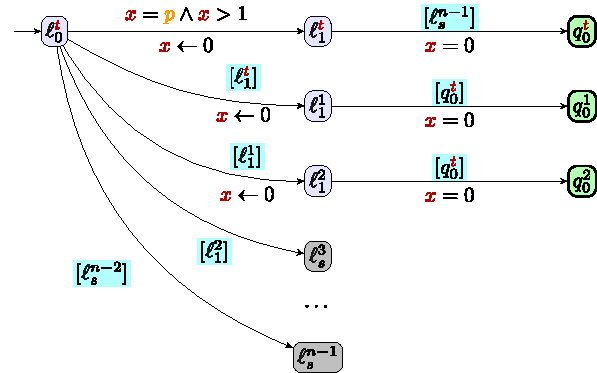
\includegraphics[width=0.95\linewidth,height=0.4\textheight,keepaspectratio]{graphic-16.pdf}\end{center}
 
Figure 5: Modified initial gadget for exactly $n$ processes.\par
 
% END A1.F5
 
% BEGIN A1.SS2.SSS0.P0.SPx1.p2
 
The rest of the proof then follows the reasoning of the proof of Proposition 14. $\hfill\blacktriangleleft$\par
 
% END A1.SS2.SSS0.P0.SPx1.p2
 
% END A1.SS2.SSS0.P0.SPx1
 
% END A1.SS2
 
% BEGIN A1.SS3
 
\par\medskip\noindent\textbf{A.3 Proof of Theorem 16}\par
 
% BEGIN A1.SS3.p1
 
% BEGIN Thmtheorem16
 
\par\medskip\noindent\textbf{Theorem 16. [Restated, see original statement.]}\par
 
% BEGIN Thmtheorem16.p1
 
PR-emptiness is undecidable for general PDTNs, even with a single clock and a single parameter (with invariants).\par
 
% END Thmtheorem16.p1
 
% END Thmtheorem16
 
% END A1.SS3.p1
 
% BEGIN A1.SS3.SSS0.P0.SPx1
 
\par\medskip\noindent\textbf{Proof.}\par
 
% BEGIN A1.SS3.SSS0.P0.SPx1.p1
 
First note that, in order to traverse the gadgets from the proof of Proposition 13, one needs (at least) 3 processes, due to the interdependency between the location guards. We will show that any process beyond the 3 required processes can only “mimic” the behaviour of one of the 3 required processes.\par
 
% END A1.SS3.SSS0.P0.SPx1.p1
 
% BEGIN A1.SS3.SSS0.P0.SPx1.p2
 
Consider a process beyond the first three processes. In the initial gadget (Figure 2(e)), it can “choose” any of the three branches leading to the three subparts, as the first three processes make them all available.\par
 
% END A1.SS3.SSS0.P0.SPx1.p2
 
% BEGIN A1.SS3.SSS0.P0.SPx1.p3
 
First assume this extra process follows the first subpart, simulating clock $t$: observe that, in all the gadgets of the first subpart (Figures 2(b), 3(b), and 4(b)), the behaviour is almost completely deterministic (e.g., all locations with invariant “$t\leq p$” are followed by a transition guarded by “$t=p$”). The only exception is in the branching to either $\mathrm{\mathrm{\ell}}_{i}^{t}$ or $\mathrm{\mathrm{\ell}}_{k}^{t}$ in Figure 4(b); assuming exactly one of the location guards $[\mathrm{\mathrm{\ell}}_{i1}^{1}]$ or $[\mathrm{\mathrm{\ell}}_{k}^{1}]$ holds (which we discuss below), then this aforementioned extra process will follow exactly the behaviour of the first process.\par
 
% END A1.SS3.SSS0.P0.SPx1.p3
 
% BEGIN A1.SS3.SSS0.P0.SPx1.p4
 
Alternatively, assume that this extra process follows the second subpart (simulating $x_{1}$) and let us show that it will follow the second process (the third subpart is similar). In most locations of our gadgets (Figures 2(c), 3(c), and 4(c)), the outgoing guards are tight w.r.t. the invariant (e.g., invariant “$x_{1}\leq p+1$” followed by a transition guarded by “$x_{1}=p+1$”), and this extra process is forced to follow the second process. In the remaining locations followed by non-tight guards (e.g., “$x_{1}\leq p$” in the increment gadget in Figure 3(c)), the guard is always additionally guarded by the location guard $[q_{j}^{t}]$, which makes its behaviour deterministic since the processes simulating clock $t$ are deterministic. Therefore, this extra process is again forced to follow the second process. The 0-test and decrement gadget is similar, with one additional crucial observation: since the aforementioned extra process mimicked the second process so far, then in $q_{i}^{1}$, due to the location guard $[q_{i}^{t}]$ ensuring a transition in 0-time, then either $x_{1}=0$ or $x_{1}>0$ holds, and therefore either both processes simulating $x_{1}$ reach $\mathrm{\mathrm{\ell}}_{i1}^{1}$, or both of them reach $\mathrm{\mathrm{\ell}}_{k}^{1}$ -- which justifies the assumption made earlier.\par
 
% END A1.SS3.SSS0.P0.SPx1.p4
 
% BEGIN A1.SS3.SSS0.P0.SPx1.p5
 
For these reasons, $q_{\textrm{halt}}$ is reachable only if the first three processes correctly simulate the 2CM; since any additional processes will just simulate one of the first three processes, we can just apply the correctness argument from the proof of Proposition 13. $\hfill\blacktriangleleft$\par
 
% END A1.SS3.SSS0.P0.SPx1.p5
 
% END A1.SS3.SSS0.P0.SPx1
 
% END A1.SS3
 
% BEGIN A1.SS4
 
\par\medskip\noindent\textbf{A.4 Proof of Theorem 17}\par
 
% BEGIN A1.SS4.p1
 
% BEGIN Thmtheorem17
 
\par\medskip\noindent\textbf{Theorem 17. [Restated, see original statement.]}\par
 
% BEGIN Thmtheorem17.p1
 
PGR-emptiness is undecidable for general PDTNs, even with a single clock and a single parameter, with or without invariants.\par
 
% END Thmtheorem17.p1
 
% END Thmtheorem17
 
% END A1.SS4.p1
 
% BEGIN A1.SS4.SSS0.P0.SPx1
 
\par\medskip\noindent\textbf{Proof.}\par
 
% BEGIN A1.SS4.SSS0.P0.SPx1.p1
 
We prove the result without invariants. (The case with invariants is simpler and follows immediately.)\par
 
% END A1.SS4.SSS0.P0.SPx1.p1
 
% BEGIN A1.SS4.SSS0.P0.SPx1.p2
 
The idea is that we ask whether all processes can reach the target location $q_{\textrm{halt}}$, which can only be done if the 2CM was properly simulated. First note that asking whether all processes can reach the target location $q_{\textrm{halt}}$ is a property satisfying the definition of global property in Section 4, by simply checking that the number of all locations but $q_{\textrm{halt}}$ is exactly 0 (called “target problem”).\par
 
% END A1.SS4.SSS0.P0.SPx1.p2
 
% BEGIN A1.SS4.SSS0.P0.SPx1.p3
 
As in the proof of Theorem 16, in order to traverse the gadgets from the proof of Proposition 13, one needs (at least) 3 processes, due to the interdependency between the location guards. We show here that any process beyond the 3 required processes can only “mimic” the behaviour of one of the 3 required processes, or block the system due to a timelock if it fails to correctly mimic it.\par
 
% END A1.SS4.SSS0.P0.SPx1.p3
 
% BEGIN A1.SS4.SSS0.P0.SPx1.p4
 
First note that if any of the first three processes does not correctly encode the 2CM (which is a possibility due to the absence of invariants), then an outgoing guard will not be firable, and therefore this process will be blocked forever in its current location, and the global property that all processes must reach $q_{\textrm{halt}}$ cannot hold. So we assume that the first three processes correctly encode the 2CM (w.l.o.g. we assume that process $i$ encodes the $i$-th subpart).\par
 
% END A1.SS4.SSS0.P0.SPx1.p4
 
% BEGIN A1.SS4.SSS0.P0.SPx1.p5
 
Now consider a process beyond the first three processes. In the initial gadget (Figure 2(e)), it can “choose” any of the three branches leading to the three subparts, as the first three processes make them all available. Due to the absence of invariants, the process can also choose to not pass the initial gadget -- but failing to take such a guard will block it forever in a location due to the guards $x=0$, and the global property that all processes must reach $q_{\textrm{halt}}$ will never hold.\par
 
% END A1.SS4.SSS0.P0.SPx1.p5
 
% BEGIN A1.SS4.SSS0.P0.SPx1.p6
 
First assume this extra process follows the first subpart, simulating clock $t$: just as in the proof of Theorem 16, because in all the gadgets of the first subpart (Figures 2(b), 3(b), and 4(b)), the guards are always punctual (i.e., involve equalities), then this extra process will either follow exactly the behaviour of the first process, or fail in taking some guard -- therefore remaining forever in its location and violating the global reachability property.\par
 
% END A1.SS4.SSS0.P0.SPx1.p6
 
% BEGIN A1.SS4.SSS0.P0.SPx1.p7
 
Alternatively, assume that this extra process follows the second subpart (simulating $x_{1}$). As in the former reasoning, either that extra process will exactly mimic the behaviour of the second process, or will fail in taking some guard, and therefore being blocked in its location, thus violating again the global reachability property.\par
 
% END A1.SS4.SSS0.P0.SPx1.p7
 
% BEGIN A1.SS4.SSS0.P0.SPx1.p8
 
The case of the final gadget is similar: if any of the processes arrive too early or too late, they will be blocked due to the urgent guards (of the form $x=0$ together with the location guards), and the global reachability will be violated.\par
 
% END A1.SS4.SSS0.P0.SPx1.p8
 
% BEGIN A1.SS4.SSS0.P0.SPx1.p9
 
For these reasons, $q_{\textrm{halt}}$ is reachable only if the first three processes correctly simulate the 2CM and if all additional processes simulate exactly one of the first three processes. Finally, we can again apply the correctness argument from the proof of Proposition 14. $\hfill\blacktriangleleft$\par
 
% END A1.SS4.SSS0.P0.SPx1.p9
 
% END A1.SS4.SSS0.P0.SPx1
 
% END A1.SS4
 
% END A1


% BEGIN A2
 
\par\medskip\noindent\textbf{Appendix B Proofs of Section 6}\par
 
% BEGIN A2.SS1
 
\par\medskip\noindent\textbf{B.1 Proof of Theorem 18}\par
 
% BEGIN A2.SS1.p1
 
% BEGIN Thmtheorem18
 
\par\medskip\noindent\textbf{Theorem 18. [Restated, see original statement.]}\par
 
% BEGIN Thmtheorem18.p1
 
PR-emptiness (resp. PGR-emptiness) for fully parametric PDTNs with 1 parameter and arbitrarily many clocks is equivalent to PR (resp. PGR) for DTNs.\par
 
% END Thmtheorem18.p1
 
% END Thmtheorem18
 
% END A2.SS1.p1
 
% BEGIN A2.SS1.SSS0.P0.SPx1
 
\par\medskip\noindent\textbf{Proof.}\par
 
% BEGIN A2.SS1.SSS0.P0.SPx1.p1
 
Let $\mathcal{A}$ be a fully parametric gPTA with 1 parameter $p$. ${\mathcal{A}}^{\infty}$ is therefore a fully parametric PDTN. Let $v_{0}$ and $v_{1}$ denote the valuations such that $v_{0}(p)=0$ and $v_{1}(p)=1$, a concept reused from the proof of [27, Corollary 4.8].\par
 
% END A2.SS1.SSS0.P0.SPx1.p1
 
% BEGIN A2.SS1.SSS0.P0.SPx1.p2
 
We prove the result for global reachability properties (PGR-emptiness), as local properties are a subcase. Fix a global property $\varphi$. Let us show that PGR-emptiness does not hold iff $\varphi$ is satisfied in a configuration reachable in ${(v_{0}(\mathcal{A}))}^{\infty}$ or in ${(v_{1}(\mathcal{A}))}^{\infty}$.\par
 
% END A2.SS1.SSS0.P0.SPx1.p2
 
% BEGIN A2.SS1.SSS0.P0.SPx1.p3
 
The following lemma derives easily from [27, Proposition 4.7], adapted to the semantics of NTAs (Section 3), and comes from the fact that, whenever no constant terms are used in a gPTA, then rescaling the parameter valuation does not impact the satisfaction of reachability properties.\par
 
% END A2.SS1.SSS0.P0.SPx1.p3
 
% BEGIN Thmtheorem21
 
\par\medskip\noindent\textbf{Lemma 21 (Multiplication of constants).}\par
 
% BEGIN Thmtheorem21.p1
 
Let $\mathcal{A}$ be a fully parametric gPTA with a single parameter $p$. Fix $n\in\mathbb{N}$. Let $\varphi$ be a global property. Then for all parameter valuations $v$, a configuration $\mathfrak{c}$ with $\mathfrak{c}\models\varphi$ is reachable in ${(v(\mathcal{A}))}^{n}$ iff $\forall t\in\mathbb{Q}_{>0}$ such that $t\times v(p)\in\mathbb{N}$, a configuration $\mathfrak{c}^{\prime}$ with $\mathfrak{c}^{\prime}\models\varphi$ is reachable in ${((t\times v)(\mathcal{A}))}^{n}$, where $t\times v$ denotes the valuation such that $(t\times v)(p)=t\times(v(p))$.\par
 
% END Thmtheorem21.p1
 
% END Thmtheorem21
 
% BEGIN A2.SS1.SSS0.P0.SPx1.p4
 
We can now proceed to the proof of Theorem 18.\par
 
% END A2.SS1.SSS0.P0.SPx1.p4
 
% BEGIN A2.SS1.SSS0.P0.SPx1.p5
  $\Rightarrow$  
% BEGIN A2.I1.ix1.p1
 
Assume PGR-emptiness does not hold for ${\mathcal{A}}^{\infty}$, i.e., there exists $v$ such that there exists $n\in\mathbb{N}_{>0}$ such that $\varphi$ is satisfied in a reachable configuration in ${(v(\mathcal{A}))}^{n}$. Let us show that $\varphi$ is satisfiable in a configuration reachable in ${(v_{0}(\mathcal{A}))}^{n}$ or in ${(v_{1}(\mathcal{A}))}^{n}$.\par
 
% END A2.I1.ix1.p1
 
% BEGIN A2.I1.ix1.p2
 
If $v(p)=0$, then the result is immediate. If $v(p)\neq 0$, then from Lemma 21, $\varphi$ is satisfied in a configuration reachable in ${(v_{1}(\mathcal{A}))}^{n}$ (by choosing some appropriate $t$, i.e., $\frac{1}{v(p)}$).\par
 
% END A2.I1.ix1.p2
  $\Leftarrow$  
% BEGIN A2.I1.ix2.p1
 
Assume $\varphi$ is satisfied in a reachable configuration in ${(v_{0}(\mathcal{A}))}^{\infty}$ or in ${(v_{1}(\mathcal{A}))}^{\infty}$. That is, there exists $n\in\mathbb{N}_{>0}$ such that there is a computation $\pi$ of ${(v_{0}(\mathcal{A}))}^{n}$ or of ${(v_{1}(\mathcal{A}))}^{n}$ reaching a configuration $\mathfrak{c}$ s.t. $\mathfrak{c}\models\varphi$. Therefore PGR-emptiness does not hold.\par
 
% END A2.I1.ix2.p1
   
Therefore, it suffices to test the satisfaction of $\varphi$ in ${(v_{0}(\mathcal{A}))}^{\infty}$ and ${(v_{1}(\mathcal{A}))}^{\infty}$.\par
 
% END A2.SS1.SSS0.P0.SPx1.p5
 
% BEGIN A2.SS1.SSS0.P0.SPx1.p6
 
Finally, the hardness argument is immediate, considering a PDTN without parameter, and replacing constants different from 1 with additional clocks and locations. $\hfill\blacktriangleleft$\par
 
% END A2.SS1.SSS0.P0.SPx1.p6
 
% END A2.SS1.SSS0.P0.SPx1
 
% END A2.SS1
 
% BEGIN A2.SS2
 
\par\medskip\noindent\textbf{B.2 Proof of Theorem 19}\par
 
% BEGIN A2.SS2.p1
 
Recall that $\mathbb{P}=\mathbb{P}_{L}\uplus\mathbb{P}_{U}$. Given $v,v^{\prime}$, we write $v^{\prime}\preceq v$ whenever $\forall p\in\mathbb{P}_{L},v^{\prime}(p)\leq v(p)$ and $\forall p\in\mathbb{P}_{U},v^{\prime}(p)\geq v(p)$.\par
 
% END A2.SS2.p1
 
% BEGIN Thmtheorem22
 
\par\medskip\noindent\textbf{Lemma 22 (Monotonicity).}\par
 
% BEGIN Thmtheorem22.p1
 
Let $\mathcal{A}$ be an L/U-gPTA. Let $v$ be a parameter valuation. For any $v^{\prime}$ such that $v^{\prime}\preceq v$, for any $n\in\mathbb{N}_{>0}$, any computation of ${(v(\mathcal{A}))}^{n}$ is a computation of ${(v^{\prime}(\mathcal{A}))}^{n}$.\par
 
% END Thmtheorem22.p1
 
% END Thmtheorem22
 
% BEGIN A2.SS2.SSS0.P0.SPx1
 
\par\medskip\noindent\textbf{Proof.}\par
 
% BEGIN A2.SS2.SSS0.P0.SPx1.p1
 
From the fact that any valuation $v^{\prime}\preceq v$ will only add behaviours due to the enlarged guards. $\hfill\blacktriangleleft$\par
 
% END A2.SS2.SSS0.P0.SPx1.p1
 
% BEGIN A2.SS2.SSS0.P0.SPx1.p2
 
% BEGIN Thmtheorem19
 
\par\medskip\noindent\textbf{Theorem 19. [Restated, see original statement.]}\par
 
% BEGIN Thmtheorem19.p1
 
PR-emptiness (resp. PGR-emptiness) for L/U-PDTNs is equivalent to PR (resp. PGR) for DTNs.\par
 
% END Thmtheorem19.p1
 
% END Thmtheorem19
 
% END A2.SS2.SSS0.P0.SPx1.p2
 
% END A2.SS2.SSS0.P0.SPx1
 
% BEGIN A2.SS2.SSS0.P0.SPx2
 
\par\medskip\noindent\textbf{Proof.}\par
 
% BEGIN A2.SS2.SSS0.P0.SPx2.p1
 
We prove the result for global reachability properties (PGR-emptiness), as local properties are a subcase. Let $\mathcal{A}$ be an L/U-gPTA and $\varphi$ a global reachability property over $\mathcal{A}$. ${\mathcal{A}}^{\infty}$ is therefore an L/U-PDTN. Consider the DTN ${(v_{0/\infty}(\mathcal{A}))}^{\infty}$. Let us show that PGR-emptiness does not hold iff $\varphi$ is satisfied in a configuration reachable in ${(v_{0/\infty}(\mathcal{A}))}^{\infty}$.\par
 
% END A2.SS2.SSS0.P0.SPx2.p1
 
% BEGIN A2.SS2.SSS0.P0.SPx2.p2
  $\Rightarrow$  
% BEGIN A2.I2.ix1.p1
 
Assume PR-emptiness does not hold for ${\mathcal{A}}^{\infty}$, i.e., there exists $v$ such that there exists $n\in\mathbb{N}_{>0}$ such that $\varphi$ is satisfied in ${(v(\mathcal{A}))}^{n}$. That is, there exists a computation $\pi$ of ${(v(\mathcal{A}))}^{n}$ reaching a configuration $\mathfrak{c}$ such that $\mathfrak{c}\models\varphi$. From Lemma 22, $\pi$ is a computation of ${(v^{\prime}(\mathcal{A}))}^{n}$, for any $v^{\prime}\preceq v$. And by extension, completely removing the upper-bound guards (i.e., valuating upper-bound parameters with $\infty$) only adds behaviour, and therefore $\pi$ is a computation of ${(v_{0/\infty}(\mathcal{A}))}^{n}$. Hence $\mathfrak{c}$ is reachable in ${(v_{0/\infty}(\mathcal{A}))}^{\infty}$, and hence $\varphi$ is satisfied.\par
 
% END A2.I2.ix1.p1
  $\Leftarrow$  
% BEGIN A2.I2.ix2.p1
 
Assume there exists a configuration $\mathfrak{c}$ reachable in ${(v_{0/\infty}(\mathcal{A}))}^{\infty}$ such that $\mathfrak{c}\models\varphi$. That is, there exists $n\in\mathbb{N}_{>0}$ such that there is a computation $\pi$ of ${(v_{0/\infty}(\mathcal{A}))}^{n}$ reaching a configuration $\mathfrak{c}$ s.t. $\mathfrak{c}\models\varphi$. Now, $v_{0/\infty}$ is not a proper parameter valuation, so we need to exhibit a parameter valuation assigning to each parameter an integer value. We reuse the same concrete parameter valuation for upper-bound parameters as exhibited in [27, Proposition 4.4]: let $T^{\prime}$ be the smallest constant occurring in the L/U-gPTA $\mathcal{A}$, and let $T$ be the maximum clock valuation along $\pi$. Fix $D=T+|T^{\prime}|+1$. (We add $T^{\prime}$ to compensate for potentially negative constant terms “$d$” in guards and invariants of $\mathcal{A}$.) Since the maximum clock valuation along $\pi$ is $T$, any guard of the form $x\leq\sum_{1\leq i\leq M}\alpha_{i}\times p_{i}+d$, that was replaced with $x<\infty$ in ${(v_{0/\infty}(\mathcal{A}))}^{n}$, can be equivalently replaced with $x\leq\sum_{1\leq i\leq M}\alpha_{i}\times D+d$ without harming the satisfaction of the guard. Therefore, $\mathfrak{c}$ is reachable in ${(v_{0/D}(\mathcal{A}))}^{n}$, and hence in ${(v_{0/D}(\mathcal{A}))}^{\infty}$. Therefore, since $\mathfrak{c}\models\varphi$, PGR-emptiness does not hold.\par
 
% END A2.I2.ix2.p1
   
Therefore, deciding PGR-emptiness for L/U-PDTNs amounts to deciding satisfaction of $\varphi$ in the DTN ${(v_{0/D}(\mathcal{A}))}^{\infty}$.\par
 
% END A2.SS2.SSS0.P0.SPx2.p2
 
% BEGIN A2.SS2.SSS0.P0.SPx2.p3
 
The case of local properties follows a similar reasoning. $\hfill\blacktriangleleft$\par
 
% END A2.SS2.SSS0.P0.SPx2.p3
 
% BEGIN A2.SS2.SSS0.P0.SPx2.p4
 
\par
 
% END A2.SS2.SSS0.P0.SPx2.p4
 
% END A2.SS2.SSS0.P0.SPx2
 
% END A2.SS2
 
% END A2

\begin{thebibliography}{99}
\bibitem{bib-bib1} 
\par\noindent    Parosh Aziz Abdulla, Mohamed Faouzi Atig, and Jonathan Cederberg.  Timed lossy channel systems.  In Deepak D’Souza, Telikepalli Kavitha, and Jaikumar Radhakrishnan, editors, FSTTCS, volume 18 of LIPIcs, pages 374--386. Schloss Dagstuhl -- Leibniz-Zentrum für Informatik, 2012.  doi:10.4230/LIPIcs.FSTTCS.2012.374.  

\bibitem{bib-bib2} 
\par\noindent    Parosh Aziz Abdulla and Giorgio Delzanno.  Parameterized verification.  International Journal on Software Tools for Technology Transfer, 18(5):469--473, 2016.  doi:10.1007/s10009-016-0424-3.  

\bibitem{bib-bib3} 
\par\noindent    Parosh Aziz Abdulla, Giorgio Delzanno, Othmane Rezine, Arnaud Sangnier, and Riccardo Traverso.  Parameterized verification of time-sensitive models of ad hoc network protocols.  Theoretical Computer Science, 612:1--22, 2016.  doi:10.1016/j.tcs.2015.07.048.  

\bibitem{bib-bib4} 
\par\noindent    Parosh Aziz Abdulla, Johann Deneux, and Pritha Mahata.  Multi-clock timed networks.  In LiCS, pages 345--354. IEEE Computer Society, 2004.  doi:10.1109/LICS.2004.1319629.  

\bibitem{bib-bib5} 
\par\noindent    Parosh Aziz Abdulla and Bengt Jonsson.  Model checking of systems with many identical timed processes.  Theoretical Computer Science, 290(1):241--264, 2003.  doi:10.1016/S0304-3975(01)00330-9.  

\bibitem{bib-bib6} 
\par\noindent    Parosh Aziz Abdulla, A. Prasad Sistla, and Muralidhar Talupur.  Model checking parameterized systems.  In Edmund M Clarke, Thomas A. Henzinger, Helmut Veith, and Roderick Bloem, editors, Handbook of Model Checking, pages 685--725. Springer, 2018.  doi:10.1007/978-3-319-10575-8\_21.  

\bibitem{bib-bib7} 
\par\noindent    Rajeev Alur and David L. Dill.  A theory of timed automata.  Theoretical Computer Science, 126(2):183--235, April 1994.  doi:10.1016/0304-3975(94)90010-8.  

\bibitem{bib-bib8} 
\par\noindent    Rajeev Alur, Thomas A. Henzinger, and Moshe Y. Vardi.  Parametric real-time reasoning.  In S. Rao Kosaraju, David S. Johnson, and Alok Aggarwal, editors, STOC, pages 592--601, New York, NY, USA, 1993. ACM.  doi:10.1145/167088.167242.  

\bibitem{bib-bib9} 
\par\noindent    Étienne André.  What’s decidable about parametric timed automata?  International Journal on Software Tools for Technology Transfer, 21(2):203--219, April 2019.  doi:10.1007/s10009-017-0467-0.  

\bibitem{bib-bib10} 
\par\noindent    Étienne André, Johan Arcile, and Engel Lefaucheux.  Execution-time opacity problems in one-clock parametric timed automata.  In Siddharth Barman and Sławomir Lasota, editors, FSTTCS, volume 323 of Leibniz International Proceedings in Informatics (LIPIcs), pages 3:1--3:22. Schloss Dagstuhl -- Leibniz-Zentrum für Informatik, December 2024.  doi:10.4230/LIPIcs.FSTTCS.2024.3.  

\bibitem{bib-bib11} 
\par\noindent    Étienne André, Benoît Delahaye, Paulin Fournier, and Didier Lime.  Parametric timed broadcast protocols.  In Constantin Enea and Ruzica Piskac, editors, VMCAI, volume 11388 of Lecture Notes in Computer Science, pages 491--512. Springer, 2019.  doi:10.1007/978-3-030-11245-5\_23.  

\bibitem{bib-bib12} 
\par\noindent    Étienne André, Paul Eichler, Swen Jacobs, and Shyam Lal Karra.  Parameterized verification of disjunctive timed networks.  In Rayna Dimitrova and Ori Lahav, editors, VMCAI, volume 14499 of Lecture Notes in Computer Science, pages 124--146. Springer, 2024.  doi:10.1007/978-3-031-50524-9\_6.  

\bibitem{bib-bib13} 
\par\noindent    Étienne André, Swen Jacobs, Shyam Lal Karra, and Ocan Sankur.  Parameterized verification of timed networks with clock invariants.  In C Aiswarya, Ruta Mehta, and Subhajit Roy, editors, FSTTCS, December 2025.  To appear.  

\bibitem{bib-bib14} 
\par\noindent    Étienne André, Swen Jacobs, and Engel Lefaucheux.  Parametric disjunctive timed networks (full version).  Technical report, arXiv, 2025.  doi:10.48550/arXiv.2512.04991.  

\bibitem{bib-bib15} 
\par\noindent    Étienne André, Michał Knapik, Wojciech Penczek, and Laure Petrucci.  Controlling actions and time in parametric timed automata.  In Jörg Desel and Alex Yakovlev, editors, ACSD, pages 45--54. IEEE Computer Society, 2016.  doi:10.1109/ACSD.2016.20.  

\bibitem{bib-bib16} 
\par\noindent    Étienne André, Didier Lime, and Nicolas Markey.  Language preservation problems in parametric timed automata.  Logical Methods in Computer Science, 16(1), January 2020.  doi:10.23638/LMCS-16(1:5)2020.  

\bibitem{bib-bib17} 
\par\noindent    Étienne André, Didier Lime, and Olivier H. Roux.  Reachability and liveness in parametric timed automata.  Logical Methods in Computer Science, 18(1):31:1--31:41, February 2022.  doi:10.46298/lmcs-18(1:31)2022.  

\bibitem{bib-bib18} 
\par\noindent    Nikola Beneš, Peter Bezděk, Kim Guldstrand Larsen, and Jiří Srba.  Language emptiness of continuous-time parametric timed automata.  In Magnús M. Halldórsson, Kazuo Iwama, Naoki Kobayashi, and Bettina Speckmann, editors, ICALP, Part II, volume 9135 of Lecture Notes in Computer Science, pages 69--81. Springer, July 2015.  doi:10.1007/978-3-662-47666-6\_6.  

\bibitem{bib-bib19} 
\par\noindent    Roderick Bloem, Swen Jacobs, Ayrat Khalimov, Igor Konnov, Sasha Rubin, Helmut Veith, and Josef Widder.  Decidability of Parameterized Verification.  Synthesis Lectures on Distributed Computing Theory. Morgan \& Claypool Publishers, 2015.  doi:10.2200/S00658ED1V01Y201508DCT013.  

\bibitem{bib-bib20} 
\par\noindent    Olaf Burkart and Bernhard Steffen.  Composition, decomposition and model checking of pushdown processes.  Nordic Journal of Computing, 2(2):89--125, 1995.  

\bibitem{bib-bib21} 
\par\noindent    Giorgio Delzanno and Pierre Ganty.  Automatic verification of time sensitive cryptographic protocols.  In Kurt Jensen and Andreas Podelski, editors, TACAS, volume 2988 of Lecture Notes in Computer Science, pages 342--356. Springer, 2004.  doi:10.1007/978-3-540-24730-2\_27.  

\bibitem{bib-bib22} 
\par\noindent    Giorgio Delzanno, Arnaud Sangnier, and Gianluigi Zavattaro.  Parameterized verification of ad hoc networks.  In Paul Gastin and François Laroussinie, editors, CONCUR, volume 6269 of Lecture Notes in Computer Science, pages 313--327. Springer, 2010.  doi:10.1007/978-3-642-15375-4\_22.  

\bibitem{bib-bib23} 
\par\noindent    Javier Esparza, Mikhail A. Raskin, and Chana Weil-Kennedy.  Parameterized analysis of immediate observation Petri nets.  In Susanna Donatelli and Stefan Haar, editors, Petri Nets, volume 11522 of Lecture Notes in Computer Science, pages 365--385. Springer, 2019.  doi:10.1007/978-3-030-21571-2\_20.  

\bibitem{bib-bib24} 
\par\noindent    Pierre Ganty and Rupak Majumdar.  Algorithmic verification of asynchronous programs.  ACM Transactions on Programming Languages and Systems, 34(1):6:1--6:48, 2012.  doi:10.1145/2160910.2160915.  

\bibitem{bib-bib25} 
\par\noindent    Carlo Ghezzi, Dino Mandrioli, Sandro Morasca, and Mauro Pezzè.  A unified high-level Petri net formalism for time-critical systems.  IEEE Transactions on Software Engineering, 17(2):160--172, 1991.  doi:10.1109/32.67597.  

\bibitem{bib-bib26} 
\par\noindent    Stefan Göller and Mathieu Hilaire.  Reachability in two-parametric timed automata with one parameter is expspace-complete.  Theoretical Computer Science, 68(4):900--985, 2024.  doi:10.1007/S00224-023-10121-3.  

\bibitem{bib-bib27} 
\par\noindent    Thomas Hune, Judi Romijn, Mariëlle Stoelinga, and Frits W. Vaandrager.  Linear parametric model checking of timed automata.  Journal of Logic and Algebraic Programming, 52-53:183--220, 2002.  doi:10.1016/S1567-8326(02)00037-1.  

\bibitem{bib-bib28} 
\par\noindent    Antonia Lechner, Joël Ouaknine, and James Worrell.  On the complexity of linear arithmetic with divisibility.  In LiCS, pages 667--676. IEEE Computer Society, 2015.  doi:10.1109/LICS.2015.67.  

\bibitem{bib-bib29} 
\par\noindent    Engel Lefaucheux.  When are two parametric semi-linear sets equal?  Technical Report hal-04172593, HAL, 2024.  URL: https://inria.hal.science/hal-04172593.  

\bibitem{bib-bib30} 
\par\noindent    Li Li, Jun Sun, Yang Liu, and Jin Song Dong.  Verifying parameterized timed security protocols.  In Nikolaj Bjørner and Frank S. de Boer, editors, FM, volume 9109 of Lecture Notes in Computer Science, pages 342--359. Springer, 2015.  doi:10.1007/978-3-319-19249-9\_22.  

\bibitem{bib-bib31} 
\par\noindent    Philip Meir Merlin and David J. Farber.  Recoverability of communication protocols-implications of a theoretical study.  IEEE Transactions on Communications, 24(9):1036--1043, 1976.  doi:10.1109/TCOM.1976.1093424.  

\bibitem{bib-bib32} 
\par\noindent    Marvin L. Minsky.  Computation: Finite and infinite machines.  Prentice-Hall, Inc., Upper Saddle River, NJ, USA, 1967.  

\bibitem{bib-bib33} 
\par\noindent    Chander Ramchandani.  Analysis of asynchronous concurrent systems by timed Petri nets.  PhD thesis, Massachusetts Institute of Technology, USA, 1973.  URL: http://hdl.handle.net/1721.1/13739.  

\bibitem{bib-bib34} 
\par\noindent    Mikhail A. Raskin, Chana Weil-Kennedy, and Javier Esparza.  Flatness and complexity of immediate observation Petri nets.  In Igor Konnov and Laura Kovács, editors, CONCUR, volume 171 of LIPIcs, pages 45:1--45:19. Schloss Dagstuhl -- Leibniz-Zentrum für Informatik, 2020.  doi:10.4230/LIPIcs.CONCUR.2020.45.  

\bibitem{bib-bib35} 
\par\noindent    Luca Spalazzi and Francesco Spegni.  Parameterized model checking of networks of timed automata with Boolean guards.  Theoretical Computer Science, 813:248--269, 2020.  doi:10.1016/j.tcs.2019.12.026.  

\end{thebibliography}
\end{document}
